% \documentclass[journal = jpccck, manuscript = article]{achemso}
% \setkeys{acs}{usetitle = true}
% \usepackage{fixltx2e}
% \usepackage{float}
% \usepackage{achemso}
% \usepackage{natbib}
% \usepackage{multirow}
% \usepackage{wrapfig}
% \usepackage{times}
% \usepackage{tablefootnote}
% \usepackage{booktabs}
% \usepackage[version=3]{mhchem}  % this is a great package for formatting chemical reactions
% \usepackage{url}
% \usepackage{graphicx}  % needed for figures
% \usepackage{dcolumn}   % needed for some tables
% \usepackage{bm}        % for math
% \usepackage{amssymb}   % for math
% \usepackage{booktabs}
% \usepackage{tablefootnote}
% \usepackage{mathptmx}

% \newcommand*{\citen}[1]{%
%   \begingroup
%     \romannumeral-`\x % remove space at the beginning of \setcitestyle
%     \setcitestyle{numbers}%
%     \cite{#1}%
%   \endgroup   
% }

\chapter[Friction at ice-I$_\mathrm{h}$ / water interfaces]{Friction at ice-I$_\mathrm{h}$ / water interfaces is governed
  by solid-liquid hydrogen-bonding} 
% \author{Patrick B. Louden}
% \author{J. Daniel Gezelter} \email{gezelter@nd.edu}
% \affiliation{Department of Chemistry and Biochemistry, University of
%   Notre Dame, Notre Dame, IN 46556} 

% \keywords{ice; water; interfaces; friction; hydrogen bonding}

% \begin{document}

% \begin{tocentry}
% \center\includegraphics[width=3.25in]{ShearingTOC.pdf} 
% Simulations of ice/water interfaces suggest that interfacial friction is
% governed by the surface density of solid-liquid hydrogen bonds.
% \end{tocentry}

% \begin{abstract}
  We present evidence that the surface density of solid to liquid
  hydrogen bonds directly correlates with the solid/liquid friction of
  ice/water interfaces. Using non-equilibrium molecular dynamics
  simulations, the basal $\{0001\}$, prismatic $\{10\bar{1}0\}$,
  pyramidal $\{20\bar{2}1\}$, and secondary prism $\{11\bar{2}0\}$
  facets of ice-I$_\mathrm{h}$ were drawn through liquid water with a
  momentum flux between the solid and liquid phases. Solid to liquid
  hydrogen bonds were identified using local tetrahedral ordering of
  the water molecules. An expression for friction coefficients
  appropriate for negative slip boundary conditions is presented, and
  the computed friction of these interfaces is found to be invariant
  to the shear rate and direction of shear relative to the surface
  features. Structural and dynamic interfacial widths for all four
  facets were found to be similar, and are also independent of the
  shear rate and direction. Differences in the solid to liquid
  hydrogen bond density are explained in terms of surface features of
  the four facets.
%\end{abstract}


\section{Introduction}

Ice friction has been investigated extensively with a range
of experiments to elucidate the role of
temperature,\cite{Bowden1939,Evans1976,Roberts1981,Derjaguin1988,Liang2003,Higgins2008} sliding speed,\cite{Evans1976,Derjaguin1988,Liang2003} applied
load,\cite{Bowden1939,Oksanen1982,Derjaguin1988,Buhl2001,Baurle2006}
contact area,\cite{Bowden1939,Baurle2007} and
moisture.\cite{Calabrese1980} Kietzig \textit{et al.} performed
experiments on steel alloy rings sliding over a prepared ice
surface.\cite{Kietzig2009} They investigated the effect of surface
nanopatterning, hydrophobicity, and surface structure of the
ice-exposed slider on the ice/slider friction.
Using laser irradiation, the slider surface hydrophobicity was tuned
without changing the chemical nature of the material. Kietzig showed
that laser-induced hydrophobicity resulted in fewer capillary bridges
forming between the slider and a thin film of melted ice. This reduced
the amount of viscous shearing of the ice-melt, resulting in a lower
friction coefficient.
While ice friction experiments have focused on heterogeneous
materials,\cite{Bowden1939,Evans1976,Derjaguin1988,Liang2003,Liang2005,Baurle2006,Baurle2007,Kietzig2009,Kietzig2010}
there have also been significant advances made on understanding
ice-ice
friction.\cite{Oksanen1982,Kennedy2000,Maeno2004,Fortt2007,Fortt2011,Lishman2011,Samadashvili2013}

Experiments and computer simulations both suggest the existence of a
quasi-liquid layer (QLL) that forms at the surface of ice at
temperatures below the bulk melting point but above
235K.\cite{Kroes1992,Ikeda-Fukazawa2004,Picaud2006,Conde2008,Bartels-Rausch2014,Sancheza2017}
The formation of this layer is driven by the termination of the
periodic crystal structure. The surface molecules are not as tightly
bound to their lattice positions as molecules in the underlying ice,
and with sufficient thermal energy, these molecules reorient to
maximize hydrogen bonding. At warmer temperatures, they can also
translate along the surface.\cite{Pfalzgraff2011,Bartels-Rausch2014}
The existence of the QLL is now generally accepted as one of the
reasons that ice displays a low coefficient of sliding
friction.\cite{Dash1995,Rosenberg2005,Dash2006,Malenkov2009}

Generally, three distinct ice friction regimes have been found:
boundary friction, mixed friction, and hydrodynamic friction, and the
particular regime depends on the temperature and sliding velocity of
the
material.\cite{Bhushan2002,Kietzig2009,Kietzig2010,Persson2015,Tuononen2016}
The observed friction is the result of different physical processes in
each regime. In boundary friction, the lubricating layer of ice melt
is only a few molecules thick. This thin film is unable to support the
sliding load, and friction can be attributed to surface asperities of
the sliding material interacting with the ice surface
itself.\cite{Bhushan2002} In the mixed friction regime, the
lubricating layer is thicker than in the boundary regime, but not yet
sufficiently thick to maintain the sliding load. The QLL film reduces
solid-solid adhesion at the interface, although the lubricating layer
can also form capillary bridges with the material, resulting in a drag
force.\cite{Kietzig2009,Kietzig2010}

If the liquid layer is thick enough to support the sliding load, the
slider's surface asperities are no longer in contact with the surface
and the observed friction may be due to the capillary bridges formed
between the ice melt and the material. Under these conditions, the ice
friction is classified as hydrodynamic
friction.\cite{Kietzig2009,Kietzig2010} Thus the three regimes are
characterized by the extent that a liquid-like layer of water
mitigates the sliding load.

\begin{figure}
\includegraphics[width=4in]{Figures/QLLsketch}
\caption{\label{fig:QLLsketch} In the hydrodynamic regime, the
  friction felt by a slider on an ice surface is mediated by a
  quasi-liquid layer (QLL) that forms on the surface of the ice.
  There can be many contributions to this friction: capillary bridges
  between the material and the QLL (red), viscous drag in the liquid
  (yellow), and solid-liquid friction between the ice and the liquid
  film (green). This study concerns the last of the three
  contributions, the drag contributed by the ice-liquid interface.}
\end{figure}

Kietzig \textit{et al.} have outlined popular experimental techniques
used to investigate the coefficients of friction for a variety of
materials sliding on ice, as well as their sensitivity to temperature,
slider load, contact area, wettability and hydrophobicity of the
slider.\cite{Kietzig2010} Of particular interest, the friction
coefficients were found to increase with increasing slider
velocity. This was attributed to three physical processes; adhesion
forces between the slider's asperities and the ice surface, breaking
of capillary bridges between the slider and the ice surface, and the
viscous shearing of the ice melt across the ice surface. While teasing
apart the individual contributions has proven challenging,
Kietzig\cite{Kietzig2009} and Persson\cite{Persson2015,Tuononen2016}
have made significant progress. However, there is still very little
known about water shearing over ice surfaces. Open questions include:
how does the structure of the interface change during this process,
and what role does the presented crystal facet have in the observed
friction?

To help understand slider-ice friction in the hydrodynamic regime, we
have simulated the drag forces contributed by the interaction of the
liquid water film with the underlying ice facet. This study uses
non-equilibrium molecular dynamics (with an applied momentum flux) to
create a shear flow at the ice/water interface. The magnitude of the
momentum flux is then used to compute the solid-liquid friction for
four different facets of ice that are presented to the liquid.  We
have previously used this technique to study solid-liquid friction for
the basal and prismatic crystal facets where we observed significant
facet-dependence, and noted surface corrugations that could contribute
to these differences.\cite{Louden2013} Here, we broaden the
investigation to four common ice facets, we study significantly larger
systems for significantly longer times, a wider range of shear rates,
and we introduce a novel method for calculating solid-liquid friction
coefficients under conditions of \textit{negative} slip.

\section{Methodology}
\subsection{Construction of Ice / Water interfaces}
Ice I$_\mathrm{h}$ crystallizes in the hexagonal space group
P$6_3/mmc$, and ice crystals normally form hexagonal plates with the
basal face, $\{0001\}$, forming the top and bottom of each plate, and
the prismatic facet, $\{10\bar{1}0\}$, forming the sides.  In extreme
temperatures or low water saturation conditions, ice crystals can form
hollow columns, needles, and dendrites, exposing other crystalline
facets of the ice to the surroundings.  Among the more
commonly-observed facets are the secondary prism, $\{11\bar{2}0\}$,
and pyramidal, $\{20\bar{2}1\}$, faces.

Although bulk ice I$_\mathrm{h}$ is proton disordered, our simulations
were carried out with proton-ordered, zero-dipole crystals that expose
stripes of dangling H-atoms and lone pairs.  These initial
configurations reproduce the surface features from Buch \textit{et
  al.}\cite{Buch2008} that helped interpret sum-frequency generation
(SFG) experiments by the Schultz lab.\cite{Groenzin07} Our structures were
created starting from Structure 6 of Hirsch and Ojam\"{a}e's set of
orthorhombic representations for ice-I$_{h}$~\cite{Hirsch2004}. The
primitive unit cell was replicated in all dimensions. The crystal was
cleaved along the desired face, and two additional mutually
perpendicular cuts were made.  The crystal was reoriented so that the
initial cut was normal to the $z$-axis of the simulation cell.  The
resulting structures were extended in $x$ and $y$ to form large
exposed facets in rectangular box geometries.

Liquid water boxes were created with identical dimensions (in $x$ and
$y$) as the ice, with a $z$ dimension of three times that of the ice
block, and with a density corresponding to $1$ g / cm$^3$.  Each of
the ice slabs and water boxes were independently equilibrated to $50$K
and a pressure of $1$ atm, and the resulting systems were merged by
carving out any liquid water molecules within 3 \AA\ of any atoms in
the ice slabs.  Each of the combined ice/water systems were then
equilibrated to $225$K, which is the liquid-ice coexistence
temperature for SPC/E water~\cite{Bryk2002}. The quiescent ice / water
interfaces were then equilibrated for 10 ns, with 5 ns under a
constant temperature (NVT) integrator set to the coexistence
temperature ($225$K), followed by 5 ns under a microcanonical (NVE)
integrator.  During this time the ice was monitored for crystal growth
or melting. We observed no advancement of the ice interface into the
liquid, and no loss of crystallinity of the ice. Reference
\citen{Louden2013} contains a more detailed explanation of the
construction of similar ice/water interfaces. The resulting dimensions
as well as the number of ice and liquid water molecules contained in
each of these systems are shown in Table \ref{tab:method}.  Note that
the water molecules are not restrained in any way - molecules that
start in the liquid phase may exchange with the ice (and vice versa).

\begin{table}[h]
\centering
\caption{Sizes of the ice/water shearing simulations. \label{tab:method}}
\begin{tabular}{r|ccccc}
\toprule
 Interface & $N_\mathrm{ice}$ &
 $N_\mathrm{liquid}$ & $L_x$ (\AA) & $L_y$ (\AA) & $L_z$ (\AA) \\
\midrule
Basal  $\{0001\}$                 & 900 & 1846  & 23.87 & 35.83 & 98.64  \\
Prismatic  $\{10\bar{1}0\}$       & 3000 & 5464 & 35.95 & 35.65 & 205.77 \\
Pyramidal  $\{20\bar{2}1\}$       & 1216 & 2203 & 37.47 & 29.50 & 93.02  \\
Secondary Prism  $\{11\bar{2}0\}$ & 3840 & 8176 & 71.87 & 31.66 & 161.55 \\
%FCC solid (111)                   & 5040 & 4867 & 38.00 & 47.01 & 122.22 \\
\bottomrule
\end{tabular}
\end{table}

The SPC/E water model~\cite{Berendsen1987} has been extensively
characterized over a wide range of liquid
conditions~\cite{Arbuckle2002,Kuang2012}, and its phase diagram has
been well studied~\cite{Baez1995,Bryk2004,Sanz2004a,Fennell2005}. With
longer cutoff radii and careful treatment of electrostatics, SPC/E
mostly avoids metastable crystalline morphologies like
ice-\textit{i}~\cite{Fennell2005} and ice-B~\cite{Baez1995}, although
Sanz \textit{et al.} found that the stable polymorph for this model is
likely ice-II at this temperature and 1 bar.\cite{Sanz2004a}  The free energies and
melting
points~\cite{Baez1995,Arbuckle2002,Gay2002,Bryk2002,Bryk2004,Sanz2004a,Fennell2005,GarciaFernandez2006,Abascal2007,Vrbka2007}
of various other crystalline polymorphs have also been calculated.
Haymet \textit{et al.} have studied quiescent ice-I$_\mathrm{h}$/water
interfaces using the SPC/E water model, and have seen structural and
dynamic measurements of the interfacial width that agree well with
both experimental results and more expensive water models, although
the coexistence temperature for SPC/E is still well below the
experimental melting point of real water~\cite{Bryk2002}. Given the
extensive data and speed of this model, it is a reasonable choice even
though the temperatures required are somewhat lower than real ice /
water interfaces.

\subsection{Creating shear in molecular simulations}
The velocity shearing and scaling variant of reverse nonequilibrium
molecular dynamics (VSS-RNEMD)\cite{Kuang2012} was employed to create
shear in our simulation cells. This method performs a series of
simultaneous nonequilibrium exchanges of linear momentum and kinetic
energy between two physically separated regions of the simulation
cell. The system responds to this unphysical flux with velocity and
temperature gradients. When VSS-RNEMD is applied to bulk liquids,
transport properties like the shear viscosity, $\eta$, are easily
extracted assuming a linear response between the applied flux,
$j_z(p_x)$, and the resulting gradient,
\begin{equation}
j_z(p_x) = -\eta \left(\frac{\partial v_x}{\partial z}\right).
\end{equation}

At interfaces between dissimilar materials, the same method can be
used to extract \textit{interfacial} transport properties (e.g. the
hydrodynamic slip length or the interfacial thermal
conductance). Because the individual VSS-RNEMD exchange moves conserve
both total energy and linear momentum, the method can be ``bolted on''
to simulations in any ensemble.  A more detailed explanation of
VSS-RNEMD shearing simulations applied to ice / water interfaces can
be found in our previous work.\cite{Louden2013}

All simulations were performed using
OpenMD~\cite{Meineke2005,Gezelter2016}, with a time step of 2 fs and
periodic boundary conditions in all three dimensions. When applicable,
VSS-RNEMD moves were attempted every time step. This minimized the
magnitude of individual momentum exchanges. For all simulations,
electrostatics were handled using the damped-shifted force real-space
electrostatic kernel.\cite{Fennell2006}

\subsubsection{Shearing at ice / water interfaces}
The RNEMD exchanges that force the solid to shear through a
surrounding liquid do measurable work on the system, and this work
causes frictional heating at the interface. Close to the melting point
of the solid, this frictional heating may result in melting of the
crystal.  We are interested in the structure and dynamics of the
interface at the coexistence temperature.  Therefore, in order to
prevent melting of the ice phase, we have imposed a weak kinetic
energy flux ($J_z \sim 2.0\times 10^{-6}$~kcal
mol$^{-1}$~\AA$^{-2}$~fs$^{-1}$) normal to the interface. The
resulting thermal gradients ($< 10$~K over the length of the
simulation box) were allowed to stabilize for 5 ns, and were found to
be sufficient in keeping the interface within $\pm 1$ K of the 225~K
target during all shearing simulations.
 
Once thermal gradients had stabilized, linear momentum fluxes were
imposed coincident with the kinetic energy flux. The resulting
velocity gradients were allowed to stabilize for 1~ns before data
collection began. Four successive 1~ns simulations were performed for
each shear rate (varying from
$0.5 \rightarrow 10.0~\mathrm{~m~s}^{-1}$) . Configurations of the
systems were stored every 1~ps, and statistics on the structure and
dynamics were accumulated every 0.1~ps. Small variations in the
measured interfacial widths between successive simulations were
observed, but there was no indication of bulk melting or crystal
growth.  That is, no large scale changes in the positions of the top
and bottom interfaces were observed during the simulations.  A
representative configuration of the solvated prismatic facet being
sheared through liquid water is shown in Figure \ref{fig:Shearing}.

\begin{figure}
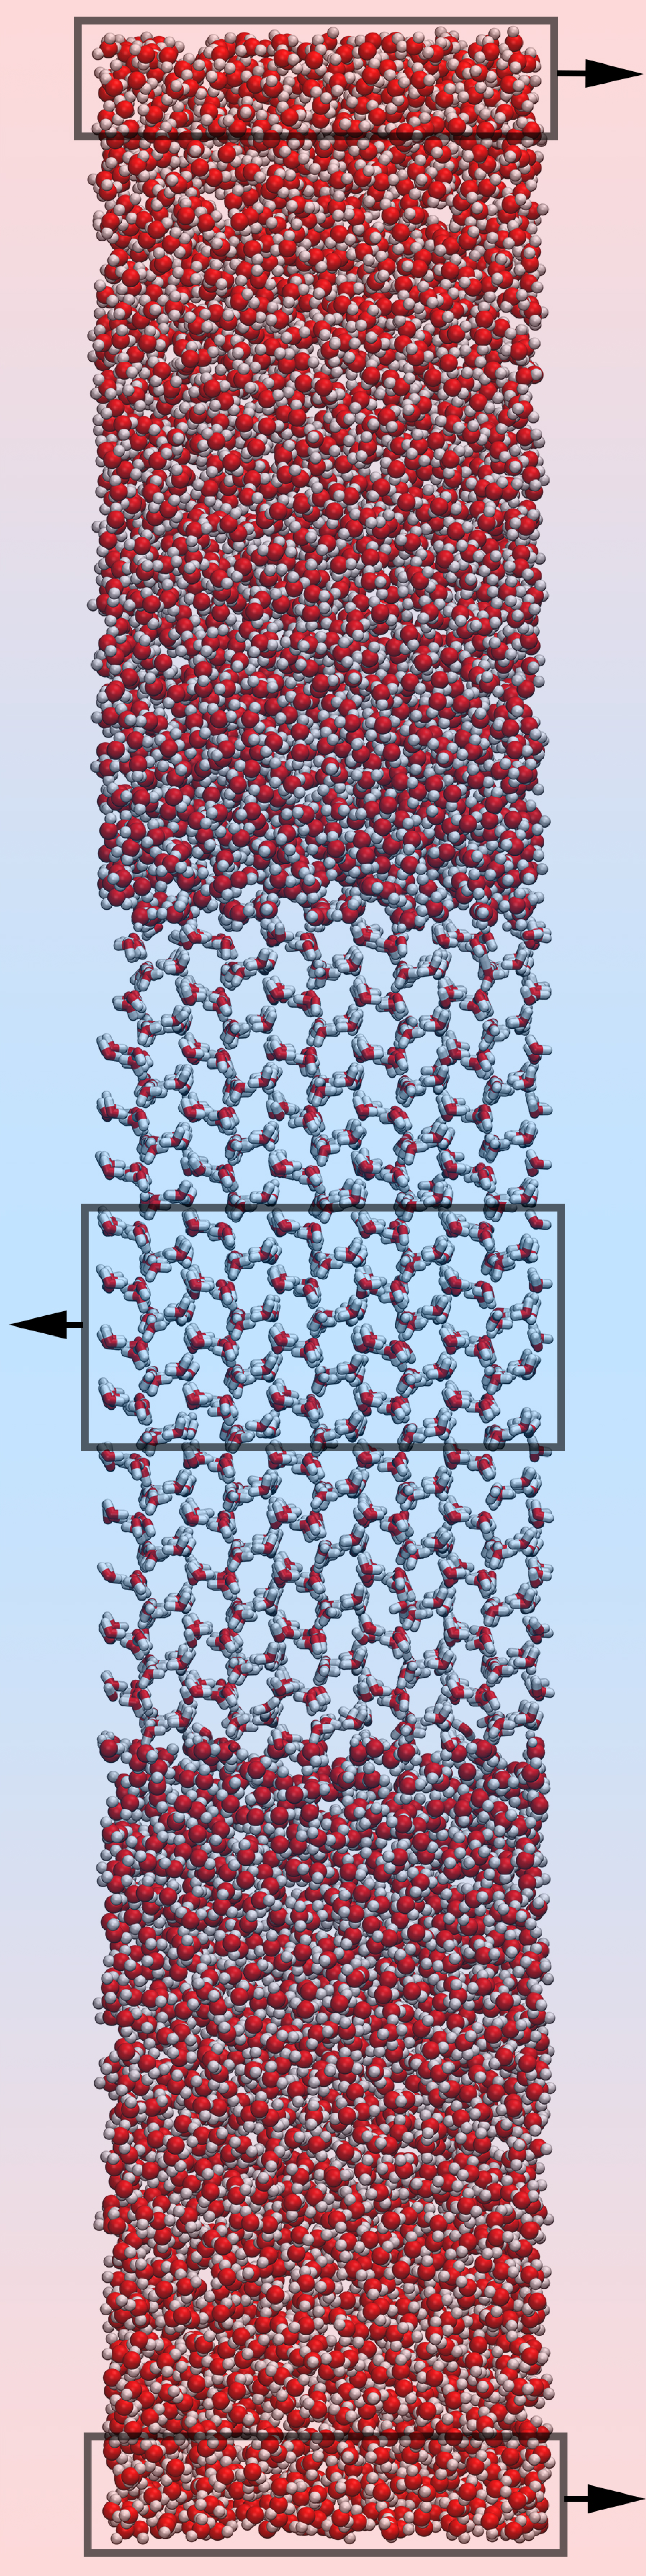
\includegraphics[width=1.9in]{Figures/Shearing}
\caption{\label{fig:Shearing} Computational model of a slab of ice
  being sheared through liquid water.  The ice presents two copies of
  the prismatic $\{10\bar{1}0\}$ facet towards the liquid phase.  The
  RNEMD simulation exchanges both linear momentum (indicated with
  arrows) and kinetic energy between the central box and the box that
  spans the cell boundary.  The system responds with weak thermal
  gradient and a velocity profile that shears the ice relative to the
  surrounding liquid.}
\end{figure}

\section{Results}

\subsection{Structural measures of interfacial width under shear}
One of the open questions about ice / water interfaces is whether the
thickness of the interfacial `slush' layer depends on the facet
of ice presented to the water. In the interfacial region, the water
molecules are ordered differently than in either the solid or liquid
phases, and also exhibit dynamics unique to their local structure.
The width of this interfacial layer has been estimated by finding the
distance over which structural order parameters or dynamic properties
change from their bulk liquid values to those of the solid ice. The
properties used to find interfacial widths have included the local
density, the diffusion constant, and both translational and
orientational order
parameters~\cite{Karim1988,Karim1990,Hayward2001,Hayward2002,Bryk2002,Gay2002,Louden2013}.

Because the VSS-RNEMD method creates thermal and velocity gradients in
the system, the momenta of the water molecules are perturbed, and
order parameters that depend on translational motion may measure the
momentum exchange and not physical properties of the interface.  As a
structural measure of the interface, we have used the local
tetrahedral order parameter, which compares the local molecular
environments (e.g. the angles between nearest neighbor molecules) to
perfect tetrahedral ordering.  This quantity was originally described
by Chau and Hardwick,~\cite{Chau1998} was rescaled by Errington and
Debenedetti,~\cite{Errington2001} and has been used in bulk liquid 
simulations by Kumar \textit{et al.}~\cite{Kumar2009} It has also
previously been used in ice/water interfaces by Bryk and
Haymet~\cite{Bryk2004}, and in our initial work on ice / water
interfaces\cite{Louden2013}.

We have evaluated the local tetrahedral order parameter, $q$, along
the coordinate perpendicular to the ice / water interface, i.e., the
$z$-axis of the simulation box.
\begin{equation}
q(z) = \frac{1}{N_z} \int_0^L \sum_{i=1}^{N} \Bigg(1 -\frac{9}{2n(n-1)}\sum_{j=1}^{n-1}
\sum_{k=j+1}^{n} \bigg(\cos\psi_{jik}+\frac{1}{3}\bigg)^2\Bigg)
\delta(z_{i}-z)\mathrm{d}z 
\label{eq:qz}
\end{equation}
$\psi_{jik}$ is the angle formed between the oxygen sites of water
molecules $i$, $j$, and $k$, where molecule $i$ is the central water
molecule and molecules $j$ and $k$ are two of the $n$ neighbors of
$i$.  Molecules $j$ and $k$ lie within the first solvation shell of
molecule $i$ ($r < 3.41$~\AA\ for water), and the double sum visits
all angles for neighbors of molecule $i$ that are within this
distance.  When molecule $i$ has exactly four neighbors ($n=4$), the
prefactor reduces to $3/8$, as in the expression of Errington and
Debenedetti, but Eq. \eqref{eq:qz} also provides tetrahedrality
information for water molecules that are either under- or
over-coordinated. We have also introduced the normalization factor
$N_z = \sum_i \int \delta(z_i - z) \mathrm{d}z$ to account for the
varying populations of water molecules within each finite-width bin.

At low temperatures, the tetrahedral order parameter can approach
unity for perfect ice-I$_\mathrm{h}$ structures. However, at
temperatures close to melting, values of 0.9 are more common due to
thermal motion in the lattice. In liquid water, overlap of the local
environment with a perfect tetrahedron is reduced, and values of
$q(z) \approx 0.75$ are common at $225$~K.

The structural widths of the ice / water interfaces were determined by
dividing each system into 1~\AA~ bins along the $z$-axis, and
computing statistical averages of $q(z)$ in each bin. For the
secondary prism interface, the resulting distribution can be seen in
the bottom panel of Fig. \ref{fig:spComic} (and in the Supporting
Information for the other interfaces). In the bulk liquid (at small
and large values of $z$), the order parameter takes on values of
$q(z) \approx~0.77$, while $q(z) \approx~0.92$ was found in bins
spanning the ice. The tetrahedrality profiles were fit using a
function that captures the smooth transition from the bulk liquid to
ice (turquoise line in the bottom panel of the same figures),
\begin{equation}\label{tet_fit}
q(z) \approx
q_\mathrm{liq}+\frac{q_\mathrm{ice}-q_\mathrm{liq}}{2}\left[\tanh\left(\frac{z-l}{w}\right)-\tanh\left(\frac{z-r}{w}\right)\right]+\beta\left|z-\frac{r+l}{2}\right|.
\end{equation}
Here $q_\mathrm{liq}$ and $q_\mathrm{ice}$ are the values of the order
parameter for the bulk liquid and ice domains. The locations $l$ and
$r$ are the $z-$coordinates of the Gibbs dividing surface for the left
and right interfaces (shown in Fig. \ref{fig:spComic} with vertical
dotted lines), and $w$ is the interfacial width.  The last term in
Eq. \eqref{tet_fit} accounts for the influence of the weak thermal
gradient on the tetrahedrality profile in the liquid region. Namely,
at warmer temperatures the liquid is able to adopt local
configurations resulting in lower values of the order parameter. This
results in a small linear decay in the tetrahedrality profiles for
increasing displacements from the ice surface.

\begin{figure}
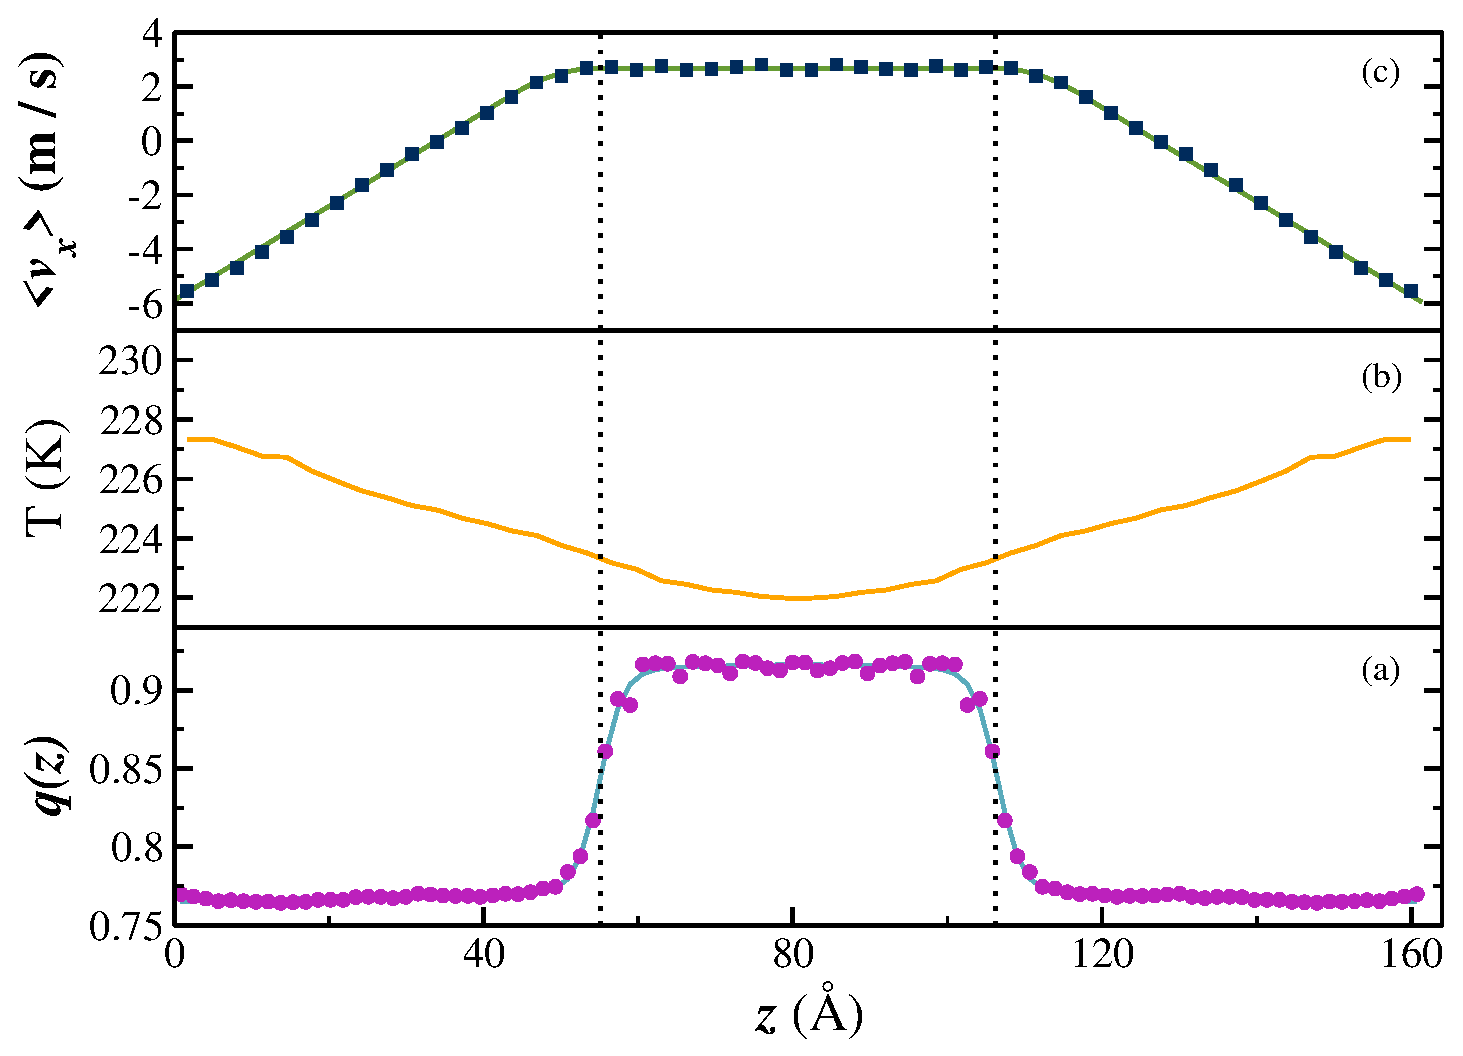
\includegraphics[width=\linewidth]{Figures/Sec_comic_strip}
\caption{\label{fig:spComic} Properties of the secondary prism
  interface being sheared through water at 8.6
  ms\textsuperscript{-1}. Lower panel: the local tetrahedral order
  parameter, $q(z)$, (circles) and the hyperbolic tangent fit
  (turquoise line).  Middle panel: the imposed thermal gradient
  required to maintain a fixed interfacial temperature of 225 K. Upper
  panel: the transverse velocity gradient (squares) that develops in
  response to an imposed momentum flux, along with the fit (green
  line). The vertical dotted lines indicate the locations of the Gibbs
  dividing surfaces of the two interfaces.}
\end{figure}

In the middle panel of Fig. \ref{fig:spComic}, we show the resulting
thermal gradient from the imposed kinetic energy flux. At the ice /
water interface, the local temperature is held at approximately 225~K, allowing
investigation of the response to the shear while maintaining
solid-liquid coexistence. In the top panel, the velocity gradient
resulting from the imposed momentum flux shows that the ice has a
uniform positive velocity along the $x$ axis. The bulk liquid at the
ends of the simulation cell has negative velocity, although the center
of mass of the simulation box is stationary.  The bulk fluid shows a
primarily linear velocity gradient allowing for easy calculation of
the shear viscosity. Close to the interface, the ice imparts
significant positive momentum into the surrounding interfacial liquid.
Projections of the velocity gradient from the liquid onto the Gibbs
dividing surface indicate that the ice-water interface is in the
negative slip regime.

From Eq. \eqref{tet_fit}, we have obtained estimates for $w$, the
structural widths of the interfaces for the quiescent ice / water
systems. These values are related to the $10\%-90\%$ interfacial
widths commonly reported in previous studies
($w_\mathrm{10-90} = 2.197~w$).\cite{Bryk2002,Bryk2004} We find
$w_\mathrm{10-90} \approx 7$~\AA~ for each of the interfaces as seen
in Table \ref{tab:kappa}.  These values are similar to our previous
findings for the $10\%-90\%$ interfacial widths obtained from shorter
simulations, ($7.0 \pm 0.9$ \AA) for the basal and ($7.9 \pm 0.4$ \AA)
for the prismatic interfaces.\cite{Louden2013} Over the range of shear
rates investigated, $\sim 0.5-10.0~\mathrm{~m~s}^{-1}$, we find no
significant differences in the interfacial widths for any of the
crystal faces. All values of $w_\mathrm{10-90}$ obtained from shearing
simulations fell inside the error bars of the values obtained from the
quiescent simulations.

\begin{table}[h]
\centering
\caption{Structural and dynamic properties of the interfaces of
  Ice-I$_\mathrm{h}$ with water.\label{tab:kappa}}
\begin{tabular}{r|cccc}  
\toprule
Interface & $w_\mathrm{10-90}$ (\AA) &  $d_\mathrm{10-90}$ (\AA) & $\kappa$ (amu \AA\textsuperscript{-2} fs\textsuperscript{-1}) & $\rho_{sl}$ (\AA\textsuperscript{-2}) \\ 
\midrule
Basal  $\{0001\}$                 & $7.5 \pm 0.4$ & $5 \pm 1$ &  $0.31 \pm 0.03$  & $0.1227 \pm 0.0003$  \\
Prismatic  $\{10\bar{1}0\}$       & $7.2 \pm 0.2$ & $8 \pm 2$  &  $0.48 \pm 0.04$  & $0.2014 \pm 0.0005$  \\
Pyramidal  $\{20\bar{2}1\}$       & $6.6 \pm 0.2$ & $6 \pm 1$ &  $0.26 \pm 0.02$  & $0.0866 \pm 0.0003$  \\
Secondary Prism  $\{11\bar{2}0\}$ & $6.7 \pm 0.2$ & $7 \pm 1$ &  $0.41 \pm 0.02$  & $0.1384 \pm 0.0004$  \\ 
\bottomrule
\end{tabular}
\end{table}

These values agree well with those reported by Haymet \textit{et
  al.}.\cite{Karim1988,Karim1990,Hayward2001,Bryk2002,Hayward2002,Bryk2004}
Using a variety of water models and several different order
parameters, they have estimated the ice / water interface to be
between $5$~\AA~and $18$~\AA~depending on the particular interface and
means of measure.  For the SPC/E model, they found the basal and
prismatic ice / water interface to be $\approx 11$~\AA~ wide from
translational and window-averaged density order parameters. The
interfacial widths were also estimated by observing the transition of
a similar tetrahedral order parameter from their ice-like value of
$0.9$ to the bulk liquid value of $0.6$. This gave estimates of
$\approx 11$~\AA~, somewhat larger than our current estimates.

\subsection{Solid-liquid friction at ice/water interfaces}
In no-stick boundary conditions, fluid flowing over a solid is
characterized by a slip length, $\delta$, describing the extent of
slip of the fluid at the interface. This length is the extrapolated
distance from the interface where the tangential velocity component
vanishes. For solids with weak interactions with the liquid, there is
little drag imposed on the fluid and the resulting interfacial liquid
velocity, $\Delta v_\mathrm{slip}$, can be significant. In no-stick
boundaries, therefore, the extrapolated slip lengths are also large
(top panel of Fig. \ref{fig:slipLengthPlot}).  Balasubramanian and
Mundy have related the slip length to the interfacial friction
coefficient, 
\begin{equation}\label{kappa1}
\lambda = \frac{\eta}{\delta}
\end{equation}
where $\eta$ is the shear viscosity of the
liquid.\cite{Balasubramanian1999}

For solids that have strong interactions with the liquid, a larger
frictional drag is imposed on the fluid at the interface and the
resulting slip lengths are smaller. When the solid-liquid interactions
become large enough, the interface is best described with stick
boundary conditions, and the slip length will vanish (middle panel of
Fig. \ref{fig:slipLengthPlot}).  Stick boundaries pose a problem for
Eq.  \eqref{kappa1}, as $\lambda$ asymptotically goes to infinity as
$\delta \rightarrow 0$.  Likewise, some materials possess solid-liquid
interactions that are strong enough for the extrapolated tangential
velocity to vanish \textit{before} reaching the solid. The velocity
profile yields a negative slip length (bottom panel of Fig.
\ref{fig:slipLengthPlot}), and the solid-liquid friction coefficient
defined in Eq. \eqref{kappa1} becomes meaningless.  Ice shearing
through liquid water is in the negative slip limit. The tangential
velocity profile of the liquid extrapolates to zero several molecular
layers before reaching the solid. Thus a new friction coefficient must
be defined to describe these interfaces.

\begin{figure}
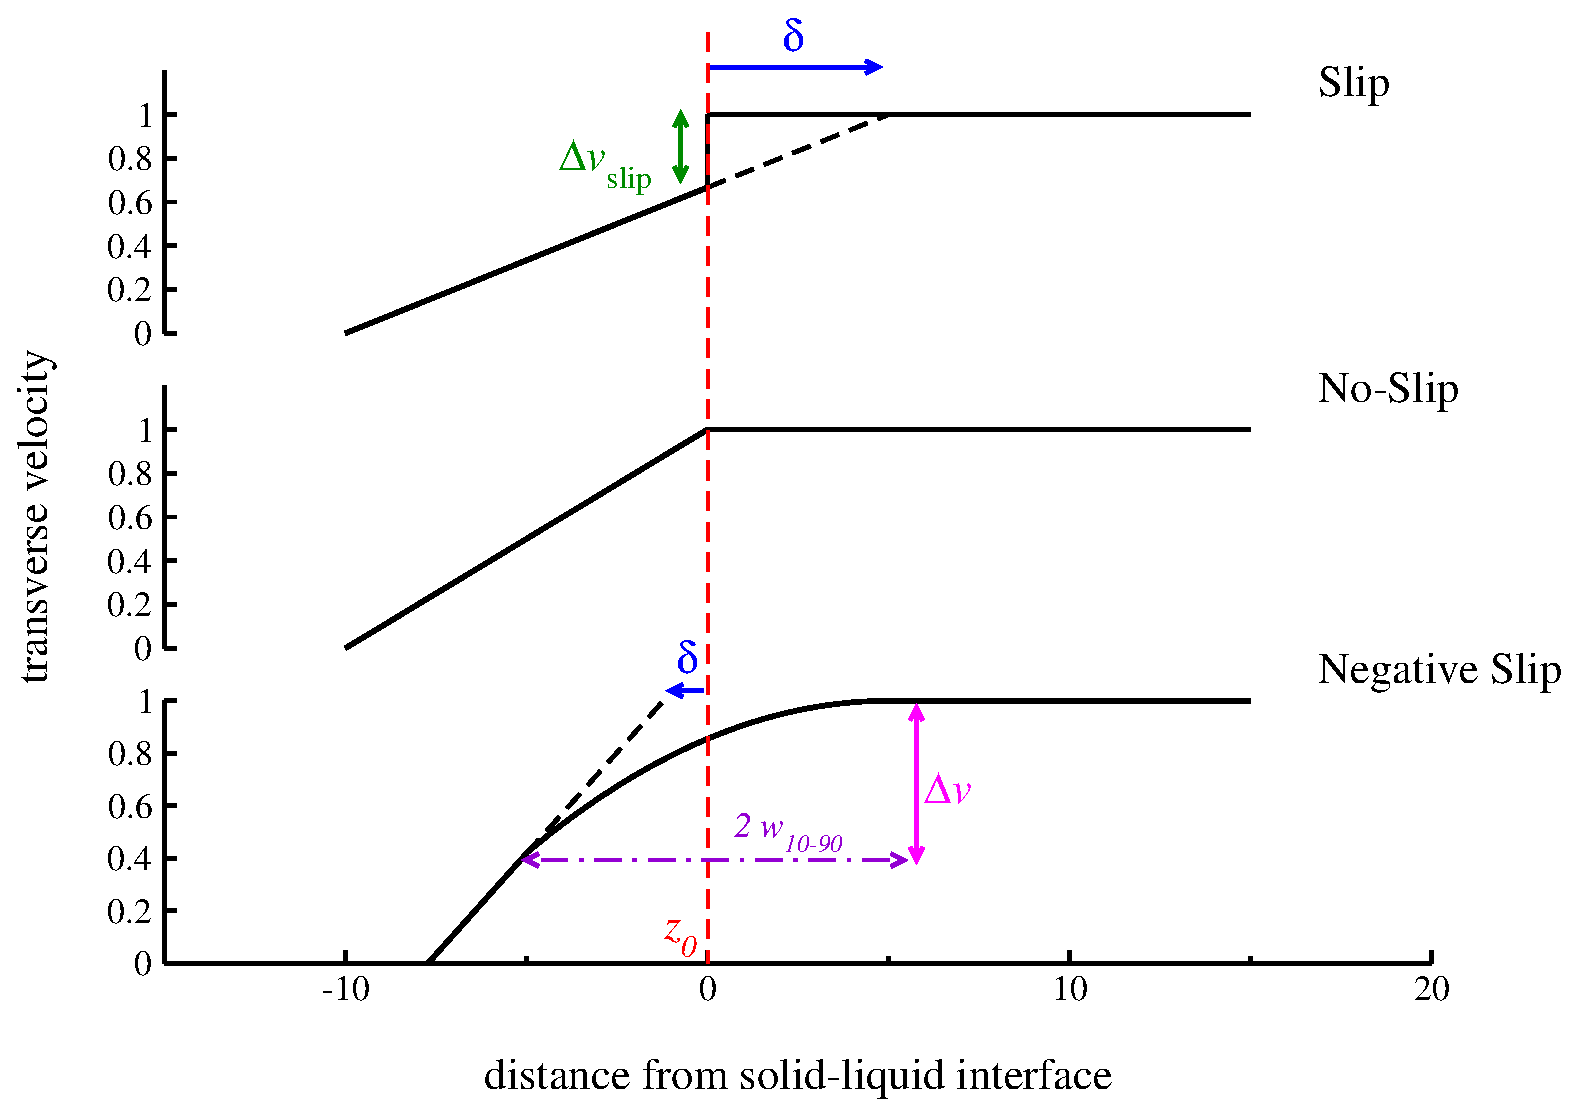
\includegraphics[width=\linewidth]{Figures/slipLengthPlot}
\caption{\label{fig:slipLength} Transverse velocity profiles,
  $v_x(z)$, for interfaces in slip (top), no-slip (middle), and
  negative slip boundary conditions (bottom).  The location of the
  interface is defined by a Gibbs dividing surface at $z_0$. Under
  negative slip conditions, the 10-90 interfacial width, $w_{10-90}$,
  provides locations that are unambiguously on the liquid and solid
  sides of the interface.\label{fig:slipLengthPlot}}
\end{figure}

The solid-liquid friction coefficient may also be defined using the
velocity drop across the interface, rather than the length scale over
which this drop occurs. We can relate the imposed shear stress with
the relative tangential velocity of the fluid in the interfacial
region,\cite{Kuang2012}
\begin{equation}\label{Shenyu-13}
j_{z}(p_{x}) = \kappa \Delta v
\end{equation}
where $\Delta v = v_{x}(\mathrm{solid}) - v_{x}(\mathrm{liquid})$ is
the difference in transverse velocity between points that are
unambiguously on the solid and liquid sides of the interface.  In slip
boundary conditions, $\kappa$ and $\lambda$ are identical, but
Eq. \eqref{Shenyu-13} provides a direct analogy to non-equilibrium
expressions for the interfacial thermal conductance $(G)$,
\begin{equation}
J_z = G~ \Delta T.
\end{equation}
Here, $J_z$ is a thermal flux and the temperature drop is measured
across an interface of \textit{finite width}. By analogy, $\kappa$ is
a transport coefficient that measures interfacial momentum
conductance.

In ice/water interfaces, the solid-liquid boundary is not
an infinitely thin plane. An order parameter (the tetrahedrality) goes
smoothly between the phases over a few molecular diameters.  We can
use this order parameter to find the interfacial width and define
locations in space that are unambiguously on the solid and liquid
sides of the interface.  In what follows, we have used the Gibbs
dividing surface ($z_0$) and the 10$-$90 width of the interface
($w_\mathrm{10-90}$) to arrive at physical locations for measuring
$v_{x}(solid)$ and $v_{x}(liquid)$.  These uniquely define a friction
coefficient in terms of well-defined structural features ($z_0$ and
$w_\mathrm{10-90}$) and dynamic properties ($v_{x}(z)$) of the
interface.

Tangential velocity profiles from the simulations were fit using a
piecewise function that is both continuous and continuously
differentiable (see Supporting Information). To arrive at estimates of
the interfacial velocities, these fits were queried at locations on
either side of the structural Gibbs dividing surface,
\begin{align*}
v_{x}(\mathrm{solid}) & = v_{x}( z_0 + w_\mathrm{10-90}) \\
v_{x}(\mathrm{liquid}) & = v_{x}( z_0 - w_\mathrm{10-90}).
\end{align*}
The momentum flux, $j_{z}(p_{x})$ is an imposed parameter of the
VSS-RNEMD simulations, and by using Eq. \eqref{Shenyu-13}, estimates
of interfacial friction coefficient $\kappa$ are straightforward.

The calculated $\kappa$ values found for the four crystalline facets
of ice-I$_\mathrm{h}$ investigated here are shown in Table
\ref{tab:kappa}.  These results were found to be independent of the
shear rate, as well as the direction of the shear relative to the
features on the surfaces of the facets.

Note that the values of $\kappa$ for the basal and prismatic crystal
facets in Table \ref{tab:kappa} disagree with values for interfacial
friction ($\lambda$) we previously reported.\cite{Louden2013} In our
initial report, the expression for the coefficient of friction was
derived from equation \eqref{kappa1} and the linear constitutive
relation for shear stress in a bulk fluid.  However, as described
above, sheared ice/water interfaces are in the domain negative slip
lengths. Eq. \eqref{kappa1} should only be used in slip boundary
conditions, as negative slip can yield coefficients of friction that
appear to be smaller in magnitude than the zero slip conditions. In
our previous work, the prismatic surface was found to have a larger
negative slip length than the basal face, indicating a prismatic
surface that should have been reported with a larger coefficient of
friction. If one instead uses Eq. \eqref{Shenyu-13} and interfacial
widths to compute friction, the reported values come into agreement.

\subsection{Dynamic measures of interfacial width under shear}
The spatially-resolved orientational time correlation function,
\begin{equation}\label{C(t)1}
  C_{2}(z,t)=\langle P_{2}(\mathbf{u}_i(0)\cdot \mathbf{u}_i(t))
  \delta(z_i(0) - z) \rangle,
\end{equation}
provides local information about the decorrelation of molecular
orientations in time. Here, $P_{2}$ is the second-order Legendre
polynomial, and $\mathbf{u}_i$ is the molecular unit vector that bisects
the HOH angle of molecule $i$. The angle brackets indicate an average
over all the water molecules and time origins, and the delta function
restricts the average to specific regions in the $z$-dimension. 

Recently, Laage and Hynes have determined the mechanism for water
reorientation.\cite{Laage2006,Laage2008} Using molecular dynamics
simulations, they found that water reorients by breaking a hydrogen
bond with an overcoordinated first-shell neighbor, and makes a large
angle jump to form a new hydrogen bond with an undercoordinated
second-shell neighbor.  The hydrogen bond cleavage and molecular
reorientation occur in a concerted fashion, not in successive steps as
was previously thought.  With this detailed picture, they constructed
the Extended Jump Model\cite{Laage2006,Laage2008} based on the Ivanov
Jump Model and parameters extracted from their molecular simulations;
the average jump amplitude of the rotational jump, $\theta_{0}$, and
the frequency of the jumps, $1/\tau_{0}$. After accounting for
molecular frame reorientation, the Extended Jump Model is able to
predict reorientation relaxation times, $\tau_{n}^{jump}$, which agree
with experimental results as well as estimates obtained from
simulations where fast librational motion is ignored.

In the ice crystal, decay of $C_2(z,t)$ is incomplete, while in the
liquid, correlation times are typically measured in ps. Observing the
spatial-transition between the decay regimes can define a dynamic
measure of the interfacial width.  To determine the dynamic widths of
the interfaces under shear, each of the systems were divided into bins
along the $z$ axis ($\approx$ 1 \AA\ wide) and $C_2(z,t)$ was computed
using only those molecules that were in the bin at the initial
time. For each ice / water interface investigated, the following 0.5
ns simulations were computed: quiescent simulations (where no thermal
or momentum gradient was present), simulations with only a thermal
gradient present, and simulations where both thermal and momentum
gradients were present. During these simulations, the positions and
orientations of each molecule were recorded every 100 fs.

\begin{figure}
\includegraphics[width=\linewidth]{Figures/CztImage}
\caption{\label{fig:Czt} $C_2(z,t)$ collected in 1 \AA~bins across the
  secondary prism ice/water interface. The band that experiences very
  little decay represents water molecules in the ice, while the band
  that decays quickly corresponds to bins in the liquid.  The
  correlation function presents a continuous distribution of decay
  behaviors across the interface between ice and liquid water.}
\end{figure}

Computed $C_2(z,t)$ values have previously been fit to a
triexponential decay, with three time constants:
$\tau_\mathrm{short}$, measuring the librational motion of the water
molecules, $\tau_\mathrm{middle}$, measuring the timescale for the
large angle jumps during the breaking and making of hydrogen bonds,
and $\tau_\mathrm{long}$, corresponding to the translational motion of
the water molecules.\cite{Louden2013} The Extended Jump Model also
includes three similar decay constants, however two of them are linked
and the dynamics of the decay is governed by two parameters. Since we
are interested in how the decay times and the individual contributions
may change through the interface, we have fit the $C_2(z,t)$ data
with
\begin{equation}
  C_{2}(z,t) = a~e^{-t/\tau_\mathrm{short}} + b~e^{-t/\tau_\mathrm{middle}} + 
  (1-a-b)~e^{-t/\tau_\mathrm{long}}
\label{eq:c2}
\end{equation}
where all of the decay constants are considered local functions of the
$z$ coordinate. In Fig. \ref{fig:SPorient}, the $z$-coordinate
profiles for the three decay constants, $\tau_{\mathrm{short}}$,
$\tau_{\mathrm{middle}}$, and $\tau_{\mathrm{long}}$ for the secondary prism interface
is shown, along with their fractional components of the overall total
decay, ($a$, $b$, $1-a-b$), respectively. Similar figures for the
other interfaces are provided in the Supporting Information.

In the liquid regions of all four interfaces, $\tau_\mathrm{middle}$
and $\tau_\mathrm{long}$ consistently approach $3-6$ ps and $30-40$
ps, respectively.  Both of these times increase closer to the
interface.  Conversely, $\tau_\mathrm{short}$ decreases from a
liquid-state value of $72-76$ fs approaching the interface.

The fractional contributions of the three motions to the overall decay
changes as we approach the interface as well. Far from the ice, the
librational motion and hydrogen bond breaking/making events each
contribute to about 20 percent of the total decay, whereas frame
reorientation contributes about 60 percent. As we approach the
interface, the librations and hydrogen bond dynamics both decrease in
contribution. The librations comprise approximately 15 percent of the
overall decay at the edge of the interface, whereas the hydrogen bond
contributions drop to approximately zero. In contrast, the fraction of
the total decay due to frame reorientation is shown to increase
approaching the interface.  The time constant corresponding to this
motion is seen to logarithmically increase as we approach the interface
as the molecules become more ice-like. In the ice we would expect
molecular reorientation to be incomplete, however, at the interface we
observe frame reorientation to contribute 85 percent of the overall
decay.

\newpage
\begin{figure}
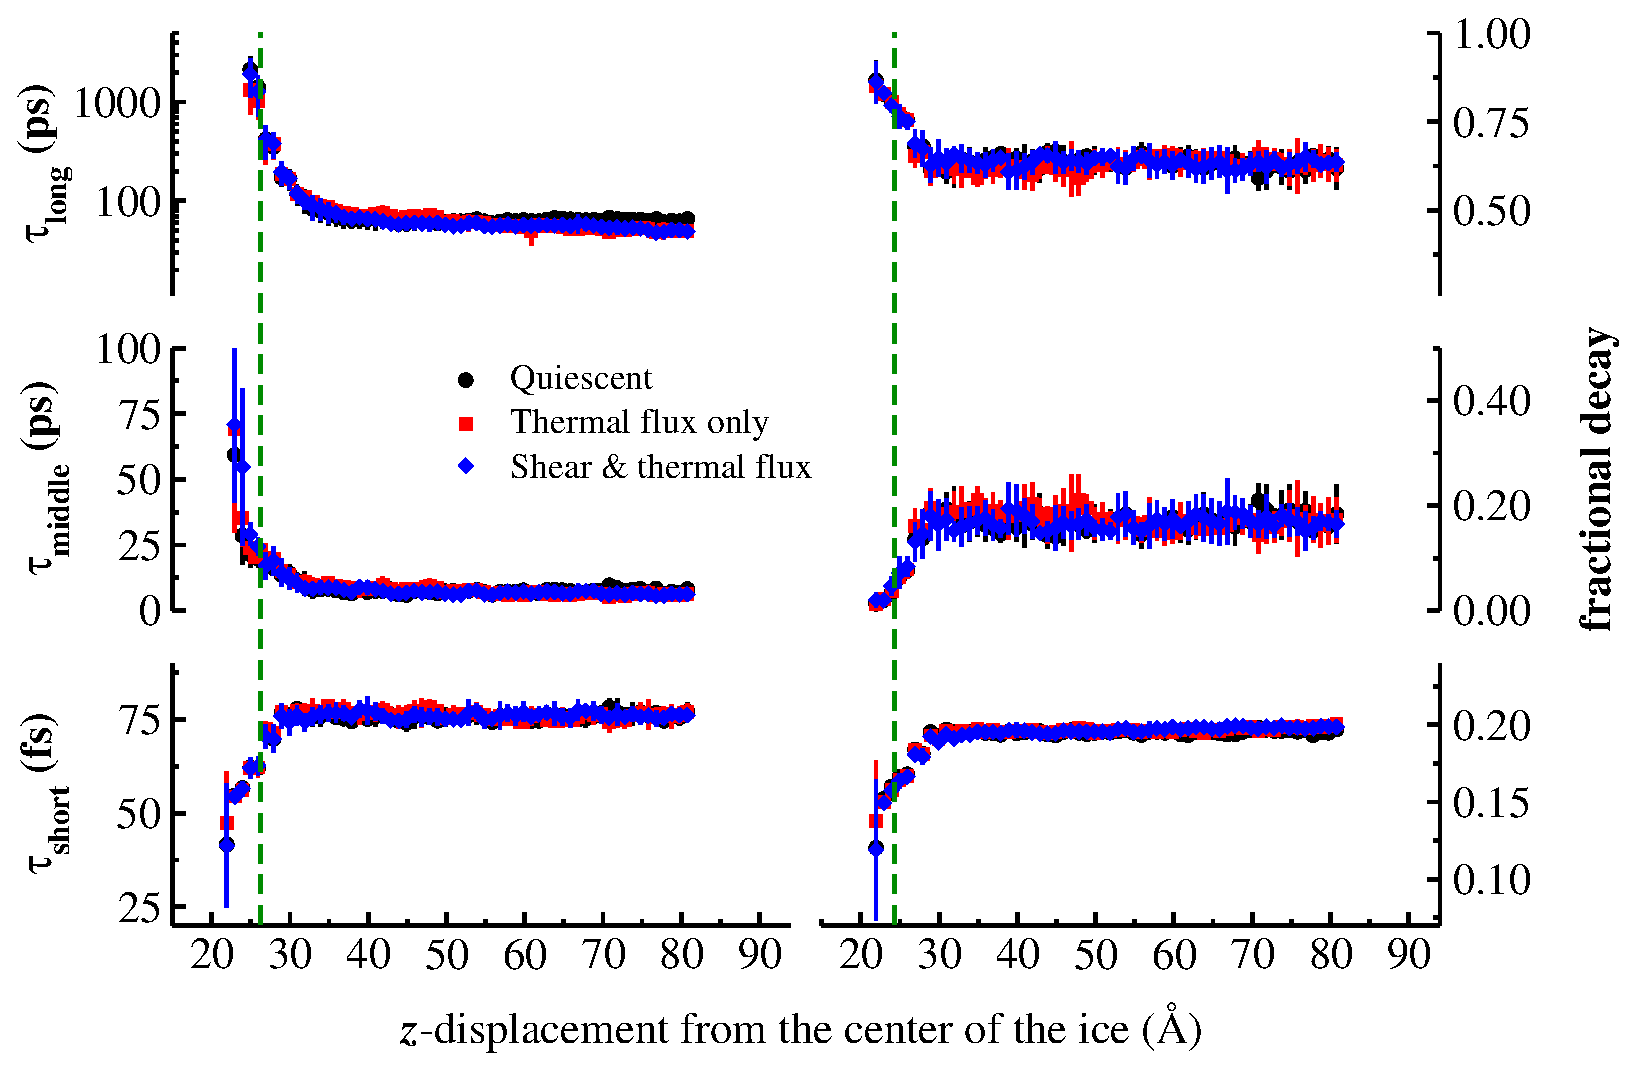
\includegraphics[width=\linewidth]{Figures/Sec_lcorrz}
\caption{\label{fig:SPorient} Decay times (left) for $C_2(z,t)$ at the
  secondary prism interface, and their fractional contributions to the
  overall decay (right) fit using Eq. \eqref{eq:c2}. The local decay
  constants are plotted as a function of distance from the center of
  the ice slab. The vertical dashed line indicates the Gibbs dividing
  surface determined using the local tetrahedral order parameter.
  Results are shown for a quiescent system with no applied kinetic or
  momentum flux (black), an interface with an imposed
  kinetic energy flux (red), and a sheared simulation (blue) with both
  kinetic and momentum fluxes.}
\end{figure}

We have estimated a dynamic interfacial width by fitting the profiles
of all the three orientational time constants with an exponential
decay to the bulk-liquid behavior,
\begin{equation}\label{tauFit}
  \tau(z) = \tau_\mathrm{liquid}+(\tau_\mathrm{wall}-\tau_\mathrm{liquid})e^{-(z-z_{0})/d}
\end{equation}
where $\tau_\mathrm{liquid}$ and $\tau_\mathrm{wall}$ are the liquid
and projected interfacial values of the decay constants, $z_{0}$ is
the location of the Gibbs dividing surface, as measured by the
structural order parameter.  As with the structural widths,
$10\%-90\%$ dynamic widths are easily computed from the fits
($d_\mathrm{10-90} = 2.197~d$).  These values are provided in Table
\ref{tab:kappa}. All four interfaces exhibit dynamic widths that are
$\sim 6$~\AA, and are in reasonable agreement with the structural
widths above.

We note that Bryk and Haymet also calculated the orientational time
correlation function at the basal interface of SPC/E
water,\cite{Bryk2002} and observed the same qualitative trend through
the ice / water interface, although the spatial resolution was not
sufficient to resolve a dynamic width.
 
Laage and Hynes investigated how water molecules reorient around
ions\cite{Laage2007,Laage2008a,Stirnemann2011a,Laage2011},
proteins\cite{Duboue-Dijon2014}, and in confined
spaces\cite{Laage2012b,Fogarty2014}.  They also studied how the
strength of the hydrogen bond might perturb the reorientation
dynamics,\cite{Laage2006a} and found the librational motion which
forms a cone around the O-O vector is smaller for more strongly
hydrogen bonded water This may also provide a partial explanation for
the increasing contribution of short time decay very close to the ice
surfaces.  Since the solid creates an excluded volume for the water
molecules that are in proximity to the interface, the hindered range
of motion (i.e., a smaller cone around the O-O vector) manifests as
faster librational decay.

\section{Discussion}
The primary result of this paper is the observation that the different
facets of ice-I$_\mathrm{h}$ produce significantly different
solid-liquid interfacial friction coefficients with water (see Table
\ref{tab:kappa}).  The two prismatic surfaces displayed the largest
coefficients of friction, while the basal and pyramidal facets
exhibited significantly lower friction.

The differences in friction are surprising given that densities and
molecular interactions are identical for the four interfaces and the
interfacial widths measured via both structural and dynamic features
are also nearly the same. There are few remaining surface properties
that could give rise to differences in solid-liquid friction of the
four facets, notably surface corrugation and hydrogen bonding density
at the interface. In this section we investigate the roles of these
surface features.

\subsubsection{Solid-liquid hydrogen bond density}
One reason for the observed differences in friction
coefficients is that ice surfaces may yield different densities of
hydrogen bonds that bridge the solid and liquid.  An ice surface that
forms more hydrogen bonds with the interfacial liquid would be able to
exert significant lateral forces on the liquid layer, yielding a
larger friction coefficient. To probe this possibility, we have
investigated the density of cross hydrogen bonds between the ice and
the liquid.

Quantifying water molecules as ``ice'' or ``liquid'' at an interface
of finite width requires a local order parameter for separating the
molecules.  We have again chosen the tetrahedral order parameter, $q$
and the value of at the Gibbs dividing surface $(q(z_0) \approx 0.84)$
as our partitioning criterion.  Note that some molecules have strong
tetrahedral ordering in the liquid phase, so this segregation will not
yield perfect division between ice and liquid phase molecules.

To determine if a hydrogen bond has been formed between two water
molecules, we used the geometric criteria of Luzar and
Chandler.\cite{Luzar1996} We identify a hydrogen bond between two
water molecules if their oxygen sites are within $r_{OO} < 3.5$
\AA~and the OHO bond angle is within $\theta_{OHO} < 30$ degrees.

For each of the shearing simulations performed above, a hydrogen bond
tetrahedrality matrix was constructed.  Snapshots from the shearing
trajectories were taken every $0.1$ ps, and the tetrahedrality $(q)$
value for each water molecule in the system was calculated. Hydrogen
bonds were also identified, and the tetrahedrality of the donor
$(q_{D})$ and acceptor $(q_{A})$ molecules were recorded. A
probability density of hydrogen bonds categorized by donor and
acceptor tetrahedrality, $\rho_\mathrm{HB}(q_D, q_A)$, was then
recorded.

\newpage
\begin{figure}
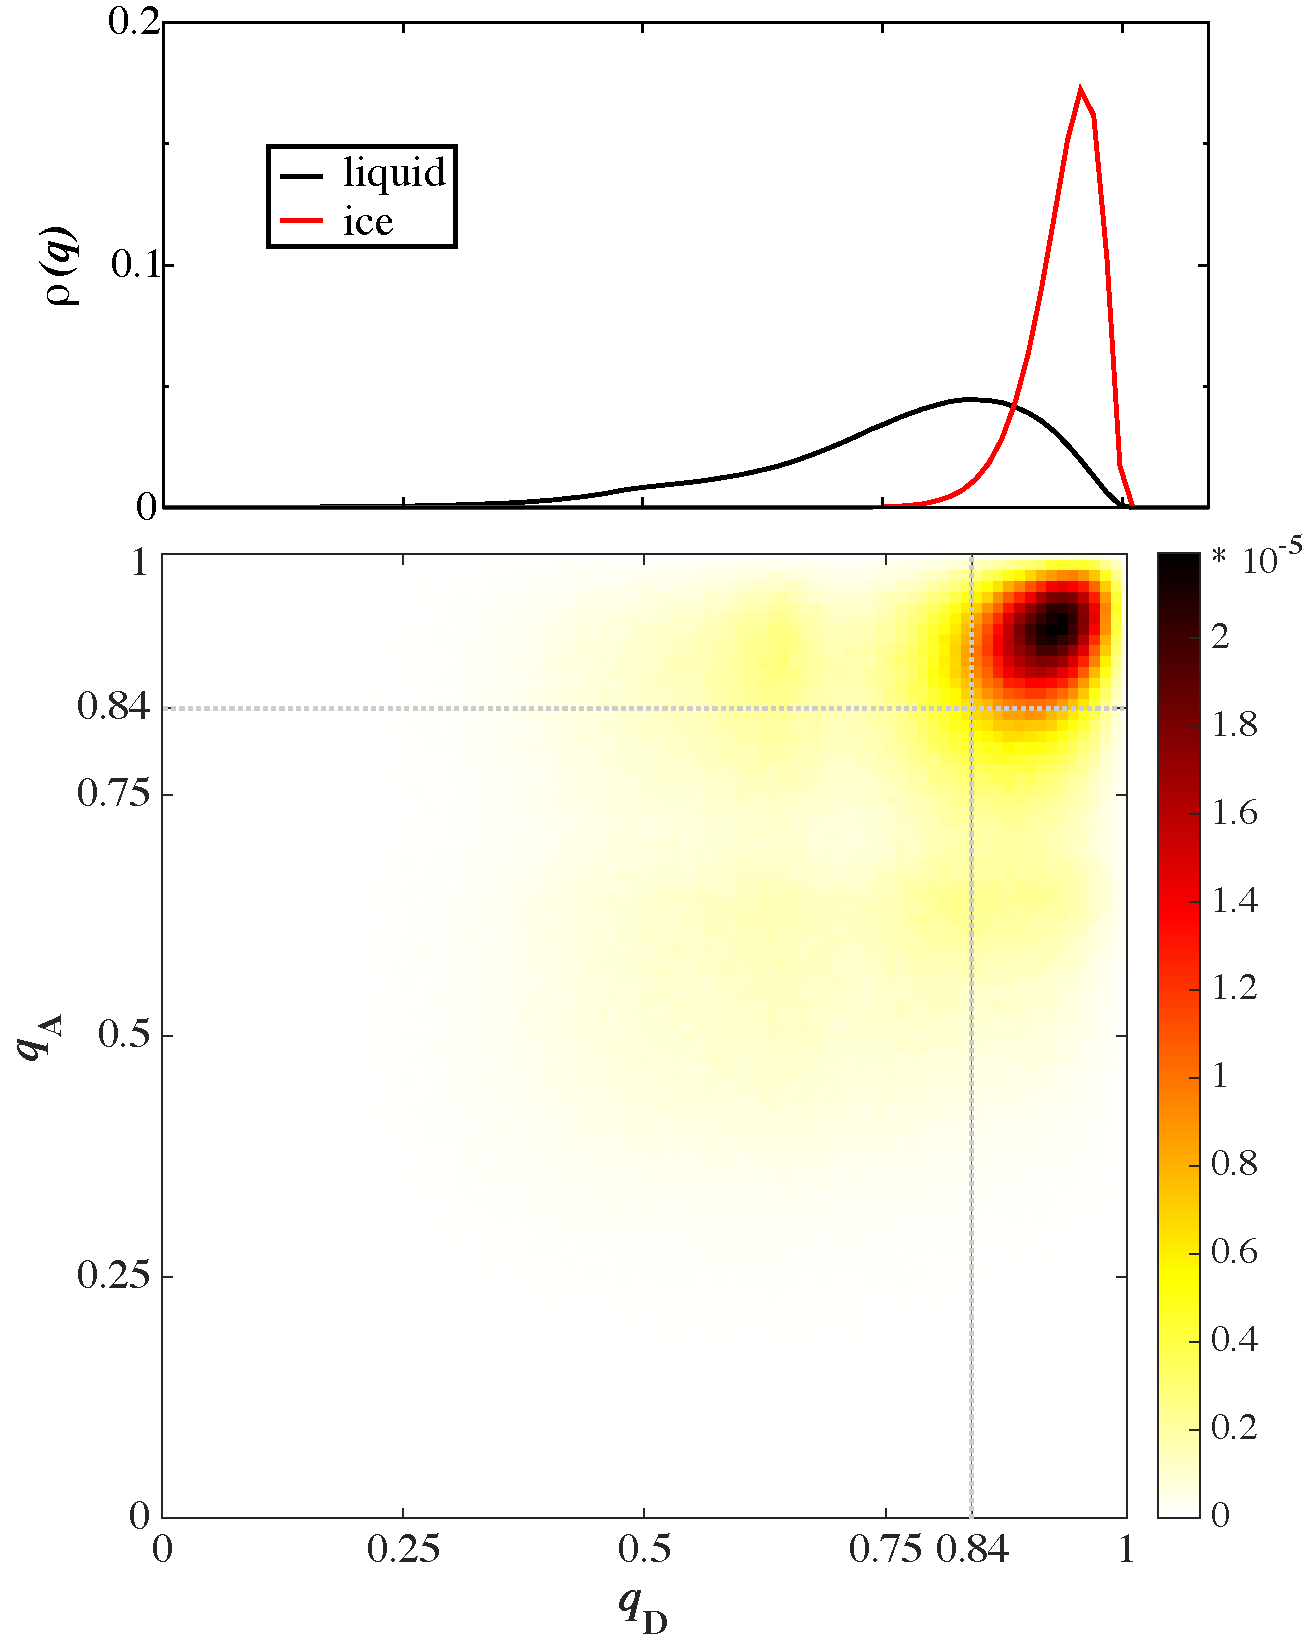
\includegraphics[width=5in]{Figures/hbtet.pdf}
\caption{\label{fig:tetHBMatrix} Distribution of hydrogen bonds at a
  prismatic interface showing the tetrahedralities of donor $(q_D)$
  and acceptor $(q_A)$ molecules (lower panel). Distributions of
  tetrahedralities in bulk ice and liquid phases are shown in the
  upper panel, and the value of $q$ at the Gibbs dividing surface is
  indicated with dashed lines. Hydrogen bonds between ice molecules
  are represented by the upper right square, while those between
  liquid molecules are in the lower left.  Hydrogen bonds that bridge
  the ice-liquid interface exist primarily in the vertical and
  horizontal strips that remain.}
\end{figure}


The lower panel of Fig. \ref{fig:tetHBMatrix} shows a hydrogen bond
tetrahedrality distribution for the prismatic facet with $q_{D}$
plotted along the $x$-axis and $q_{A}$ along the $y$-axis.  Population
around $q_{D} \approx q_{A} \approx 0.9$ indicates the density of
ice-ice hydrogen bonds in the system, while the liquid-state hydrogen
bonds are concentrated in the lower left, and are significantly more
diffuse.  The off-diagonal regions of the distribution represent the
population of molecules in tetrahedral (ice-like) environments bound
to non-tetrahedral (liquid-like) environments. Integrating the
population found in each of these regions and normalizing by the
surface area of each ice crystal produces a surface density of
hydrogen bonds (\AA\textsuperscript{-2}) formed between the ice and
interfacial liquid,
\begin{equation}\label{hbondDensity}
\rho_{sl} = \frac{N_\mathrm{HB}}{2 L_{x}L_{y}} \left[ \int_0^{0.84}
  dq_{D} \int_{0.84}^1 dq_{A}~\rho_\mathrm{HB}(q_{D},q_{A}) +  \int_0^{0.84}
  dq_{A} \int_{0.84}^1 dq_{D}~\rho_\mathrm{HB}(q_{D},q_{A}) \right]
\end{equation}
$N_\mathrm{HB}$ is the total number of hydrogen bonds found in the
system, and $L_x$ and $L_y$ are the dimensions of the two ice facets
exposed to the liquid.  Values for $\rho_{sl}$ for each of the ice
surfaces are reported in Table \ref{tab:kappa}.

The trend in surface density of solid-liquid hydrogen bonds reproduces
the trend in the friction coefficients, indicating that friction at
ice-I$_\mathrm{h}$ water interfaces is strongly influenced, if not
governed, by the number of solid-liquid hydrogen bonds that can be
formed.  This result is robust under multiple shear rates and
orientation of shear flow relative to the surface features of the ice,
indicating that the hydrogen bonding statistics between an ice facet
and the liquid are not altered by the imposed shear.

\subsubsection{Surface corrugation}
A second possible influence on the friction coefficient is the surface
topography of the ice crystals, the dimensions of which are reported
in Table \ref{tab:surf}. When a crystal of ice-I$_\mathrm{h}$ is
cleaved along either of the two prismatic crystal facets, the exposed
oxygen atoms present channel-like structures with channel widths of
6.35~\AA~ and channel depths of 2.25~\AA~.  When cleaved along the
pyramidal facet, the resulting surface features a much larger channel,
$\sim$ 8.7~\AA~ wide.  Conversely, the basal surface presents a
rather smooth surface to the liquid, with stripes of oxygen atoms
forming surface ripples with depths of $\sim$ 1.3~\AA~.

\begin{table}[h]
\centering
\caption{Surface features of Ice-I$_\mathrm{h}$ facets.\label{tab:surf}}
\begin{tabular}{r|cc}  
\toprule
Interface & Channel width (\AA) & Channel depth (\AA) \\ 
\midrule
Basal  $\{0001\}$                 & 4.49 & 1.30 \\
Prismatic  $\{10\bar{1}0\}$       & 6.35 & 2.25 \\
Pyramidal  $\{20\bar{2}1\}$       & 8.65 & 2.59 \\
Secondary Prism  $\{11\bar{2}0\}$ & 6.35 & 2.25 \\ 
\bottomrule
\end{tabular}
\end{table}

The prismatic channels are quite stable. That is, we do not observe
liquid phase molecules populating the prismatic and secondary prism
surface channels. One might expect regions of low liquid density to
yield smaller solid-liquid interactions, and it does appear that these
two surfaces present roughly half of the surface oxygen atoms to the
liquid.  However, the molecules forming the bottoms of the channels
are fully saturated (four hydrogen bonds each), while the molecules
that form the tops of the channels present a high density of available
hydrogen bond locations.

The oxygen-based surface features of the prism and secondary prism are
identical, and only the orientation of the water molecules varies.
This means that the patterning of donor and acceptors on the two
facets is quite different. A liquid with internal hydrogen bonding
constraints that is in contact with these facets will allow the
prismatic surface to form a higher density of solid-liquid hydrogen
bonds than the secondary prism, even with identical oxygen ordering at
the interface.

In contrast with the prismatic facets, liquid state molecules do
populate the surface channels on the pyramidal facet. Again, one might
expect the interactions between the solid and the liquid in close
physical contact to be quite large.  However, the liquid molecules
populating this channel do not pack efficiently and cannot fully
saturate the surface locations available for hydrogen bonding,
resulting in a lower solid-liquid hydrogen bond density and a smaller
coefficient of friction.

With its smooth surface, one could make reasonable physical arguments
for the basal face to have either high or low friction with liquid
water. That is, liquid molecules should be able to form a fully
populated network of hydrogen bonds with the surface, as there are no
recessed surface molecules at the bottoms of deep channels, and no
channel packing constraints. In the absence of large surface
undulations, however, liquid-phase molecules should also be able to
slip over the surface easily. However, the basal facet was found to
have an intermediate friction coefficient compared with the other
facets studied here. The sensible explanation in light of the
hydrogen bonding data is simply that the surface density of
solid-liquid hydrogen bonds (however transitory) dominates the
interfacial friction.

\section{Conclusions}
RNEMD simulations of the different facets of ice being drawn through
surrounding water at the coexistence temperature indicate some
facet-dependence of solid-liquid friction.  We have defined a negative
slip interfacial friction coefficient, $\kappa$ (measured in
amu~\AA$^{-2}$ fs$^{-1}$) and find that the two prismatic facets exert
the largest drag on the surrounding liquid.  The basal facet provides
an intermediate level of drag, while the pyramidal facet has roughly
half the interfacial friction of the prismatic facet.

Using the local tetrahedral order parameter as a metric to
differentiate ice and liquid water molecules and a geometric hydrogen
bonding criteria, the friction coefficients were shown to be largely
governed by the surface density of solid-liquid hydrogen bonds
($\rho_{sl}$).  A simple linear fit for the four interfaces yields
\begin{equation}
\kappa \approx 2.1772 \mathrm{(amu~fs^{-1})} \times \rho_{sl} \mathrm{(\AA^{-2})}  + 0.0777 \mathrm{(amu~\AA^{-2}~fs^{-1})},
\end{equation}
so the majority of the calculated solid-liquid friction is determined
by the surface density of solid-liquid hydrogen bonds.

In addition, we have found the ice / water interfacial widths for all
four crystal facets to be similar (using both structural and dynamic
measures) and found these widths to be independent of shear rate.  The
similarity of interfacial width estimates for the four facets indicate
that the particular facet of the exposed ice crystal has very little
effect on how far into the bulk the ice-like structural ordering
persists.  While differences have been found in previous simulations
of ice / water interfaces\cite{Hayward2001,Hayward2002},
experimentally these differences have been less
clear.\cite{Beaglehole1993} The significant differential friction
coefficients obtained here suggest that while the liquid next to the
ice might be structurally organized like bulk liquid, the dynamics of
the molecules are still quite strongly perturbed by the ice.  That is,
the surface hydrogen bonding significantly alters how the water layers
are pulled along with the ice during shear.



\section{Fitting velocity profiles}
%%%%% All this goes in SI:
In order to calculate solid-liquid friction coefficients, $\kappa$
from Eq. (5) in the main text, the velocity profiles, $v_x(z)$,
obtained from each shearing simulation were fit assuming linear
behavior through each of the three regions of the simulation box; the
lower liquid, the solid, and the upper liquid. Parabolic functions
were designed to capture the negative slip behavior that links the
three regions,
\begin{equation}\label{vfit}
v(z) =
\begin{cases}
  v_{l} - m_{l}z & 0 \leq z < (z_{1} - w) \\
  v_{s} - \frac{1}{2}k(z-z_{1})^{2} & (z_{1}-w) \leq z < z_{1} \\
  v_{s}  & z_{1} \leq z < z_{2} \\
  v_{s} - \frac{1}{2}k(z-z_{2})^{2}  & z_{2} \leq z <( z_{2} + w)\\
  v_{s} - \frac{1}{2}kw^{2} - m_{l}(z-(z_{2} + w)) & (z_{2} + w) \leq z \\
\end{cases}
\end{equation}
  
Here, $v_{l}$ is the velocity of the liquid at the middle of the
liquid domain (the edge of the simulation box), and $v_{s}$ is the
velocity of the solid. The locations $z_{1}$ and $z_{2}$ are the edges
of the ice slab, and $w$ is the width of the interface (distinct from
$w_{10-90}$ mentioned in the main text). The parameter $m_{l}$ is the
slope of the velocity profile in the liquid regions of the box which
is related to the liquid-state viscosity. Figure \ref{fig:pyrComic}
shows a representative velocity profile (navy squares) and fit (green
line) with the locations of $z_{1}$ and $z_{2}$ indicated as vertical
dotted lines. Once the fits were obtained, the values for
$v_{x}(solid)$ and $v_{x}(liquid)$ for Eq. (5) were sampled from the
fit. The $z$ locations used to sample the fit were determined by
structural measures. The $z$ location for $v_{x}(liquid)$ was taken to
be the Gibbs dividing surface of the interface, less the 10$-$90 width
of the interface. Similarly, the $z$ location for $v_{x}(solid)$ was
taken to be the Gibbs dividing surface plus the 10$-$90 width of the
interface.

%The following 4 figures are the z-rnemd profiles a. q(z), b. T(z), c. Px(z)      \newpage 
\begin{figure}
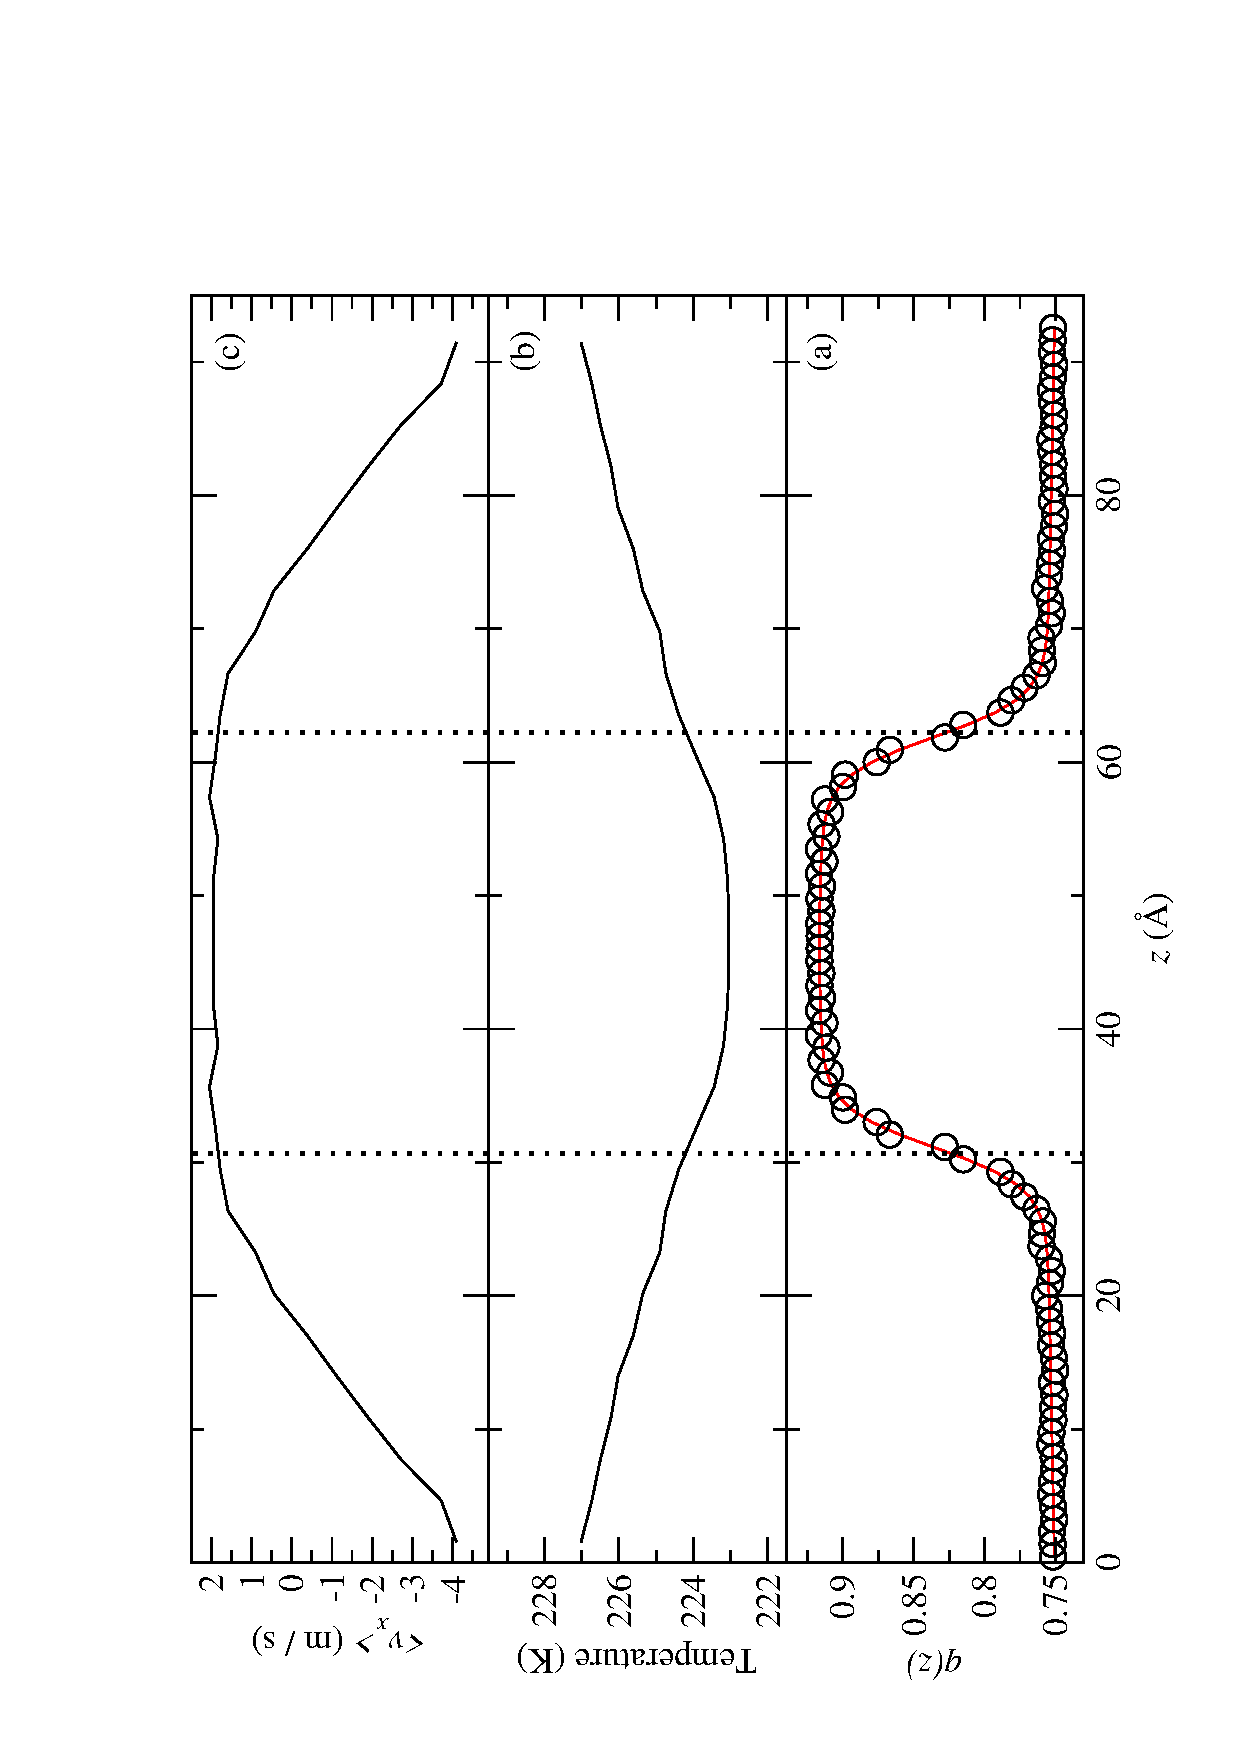
\includegraphics[width=\linewidth]{Figures/Pyr_comic_strip}
\caption{\label{fig:pyrComic} Properties of the pyramidal
  interface being sheared through water at 7.6
  ms\textsuperscript{-1}. Lower panel: the local tetrahedral order
  parameter, $q(z)$, (circles) and the hyperbolic tangent fit
  (turquoise line).  Middle panel: the imposed thermal gradient
  required to maintain a fixed interfacial temperature of 225 K. Upper
  panel: the transverse velocity gradient (squares) that develops in
  response to an imposed momentum flux, along with the fit (green
  line). The vertical dotted lines indicate the locations of the Gibbs
  dividing surfaces of the two interfaces.}
\end{figure}

\begin{figure}
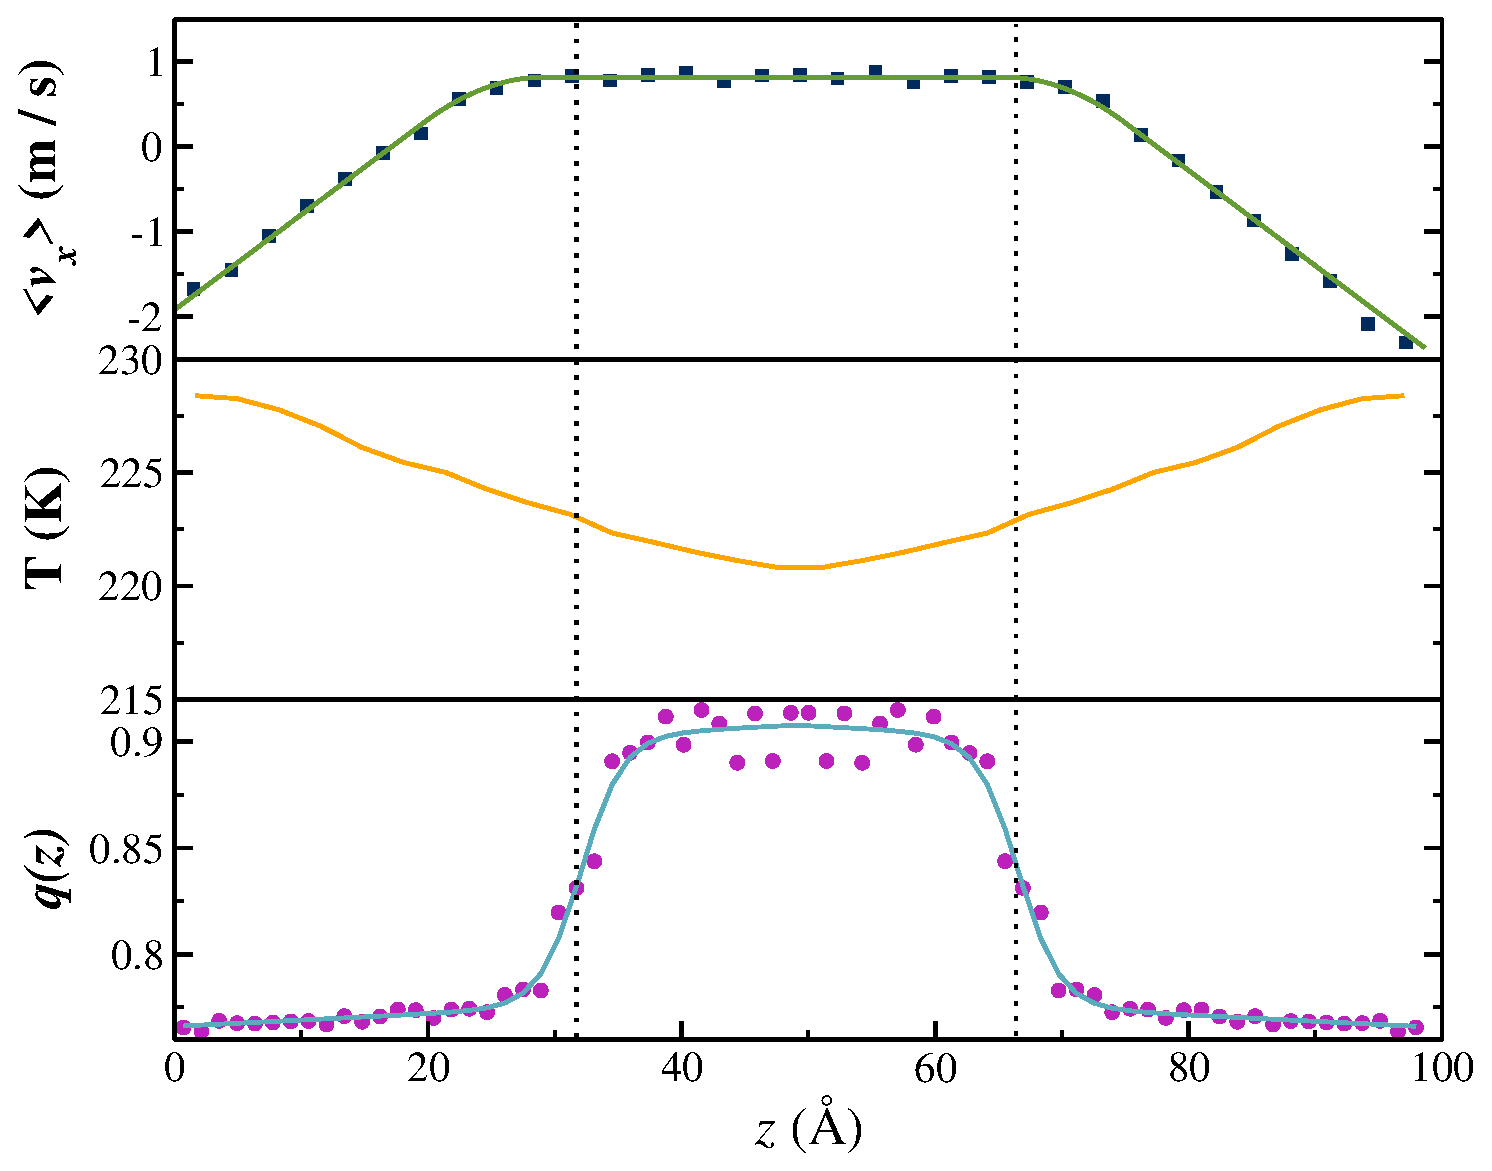
\includegraphics[width=\linewidth]{Figures/Bas_comic_strip}
\caption{\label{fig:bComic} Properties of the basal interface being
  sheared through water at 3.2 ms\textsuperscript{-1}.  Panel
  descriptions are the same as in Fig. \ref{fig:pyrComic}.}
\end{figure}

\begin{figure}
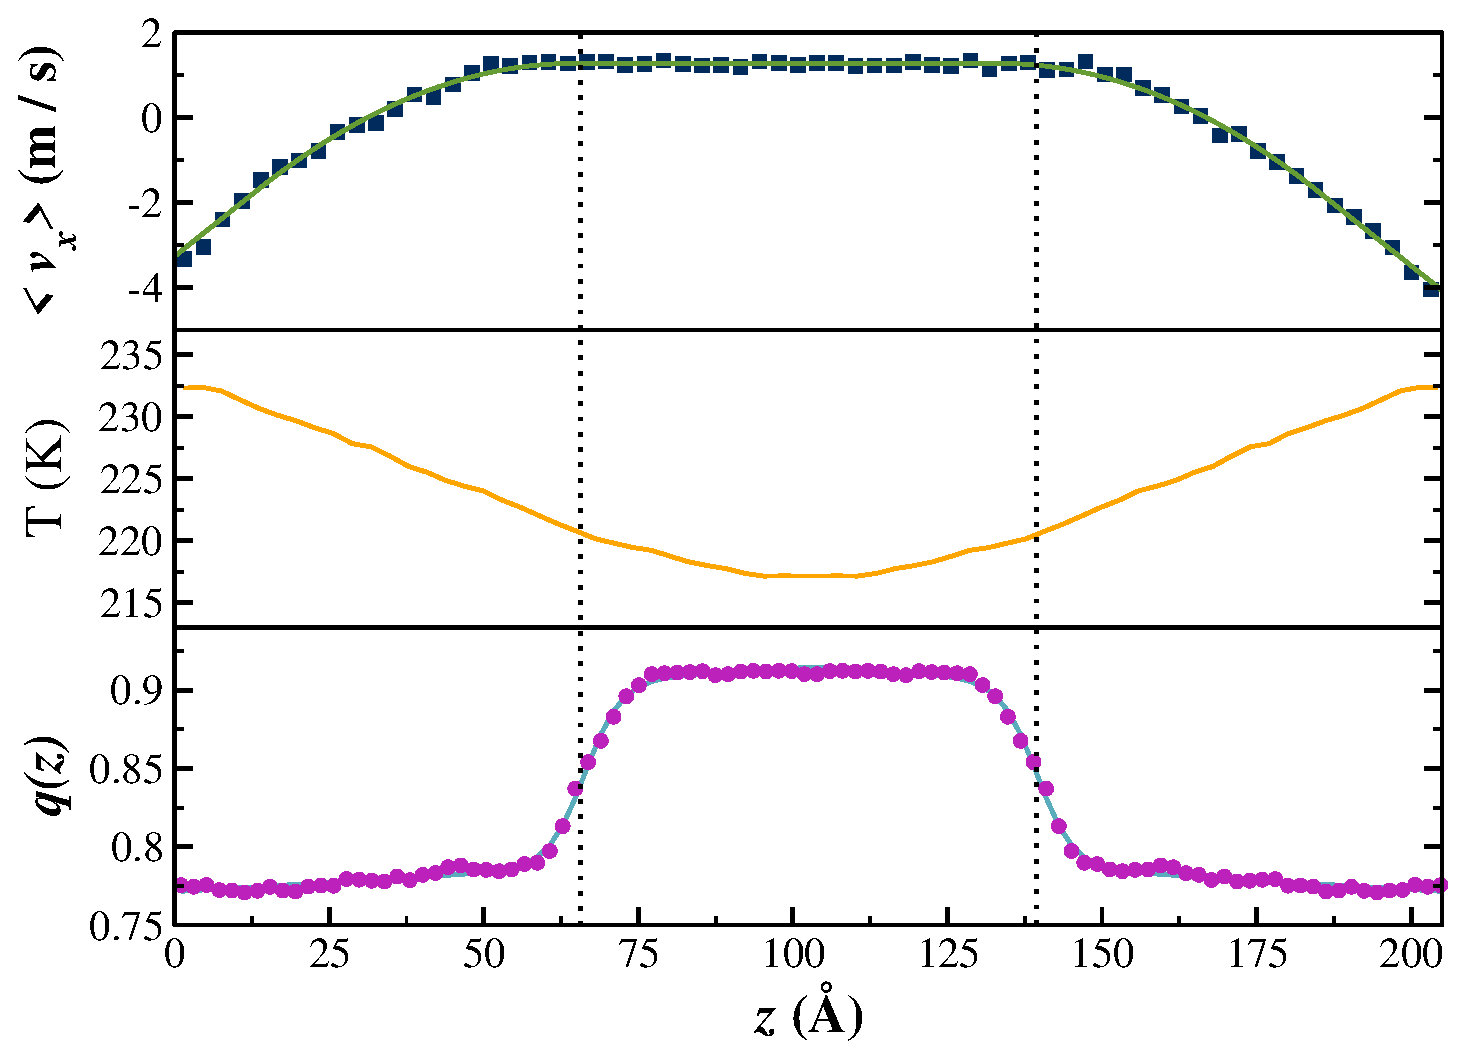
\includegraphics[width=\linewidth]{Figures/Pri_comic_strip}
\caption{\label{fig:pComic} Properties of the prismatic interface
  being sheared through water at 6.0 ms\textsuperscript{-1}.  Panel
  descriptions are the same as in Fig. \ref{fig:pyrComic}.}
\end{figure}
%End figures of z-rnemd profile. 


%Begin z-orientation times                                                         
\begin{figure}
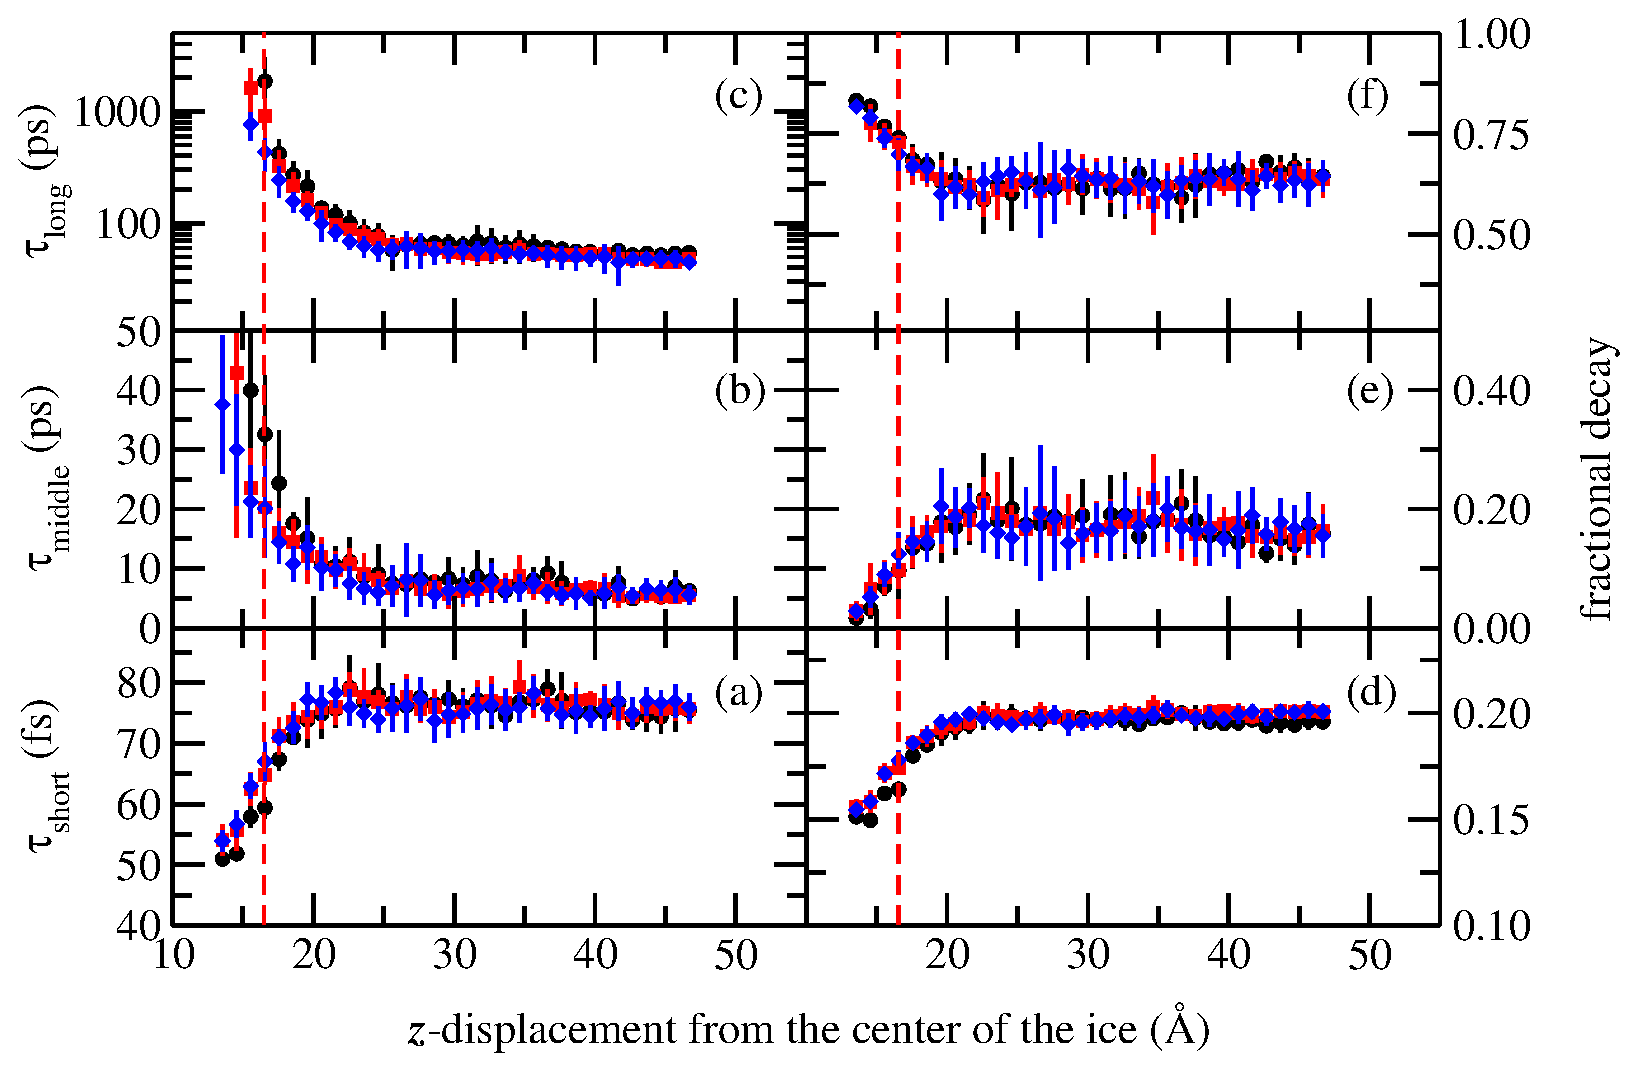
\includegraphics[width=\linewidth]{Figures/Pyr_lcorrz}
\caption{\label{fig:Pyrorient} Decay times (left) for $C_2(z,t)$ at
  the pyramidal interface, and their fractional contributions to the
  overall decay (right) fit using Eq. (8). The local decay constants
  are plotted as a function of distance from the center of the ice
  slab. The vertical dashed line indicates the Gibbs dividing surface
  determined using the local tetrahedral order parameter.  Results are
  shown for a quiescent system with no applied kinetic or momentum
  flux (black), an interface with with an imposed kinetic energy flux
  (red), and a sheared simulation (blue) with both kinetic and
  momentum fluxes.}
\end{figure}

\begin{figure}
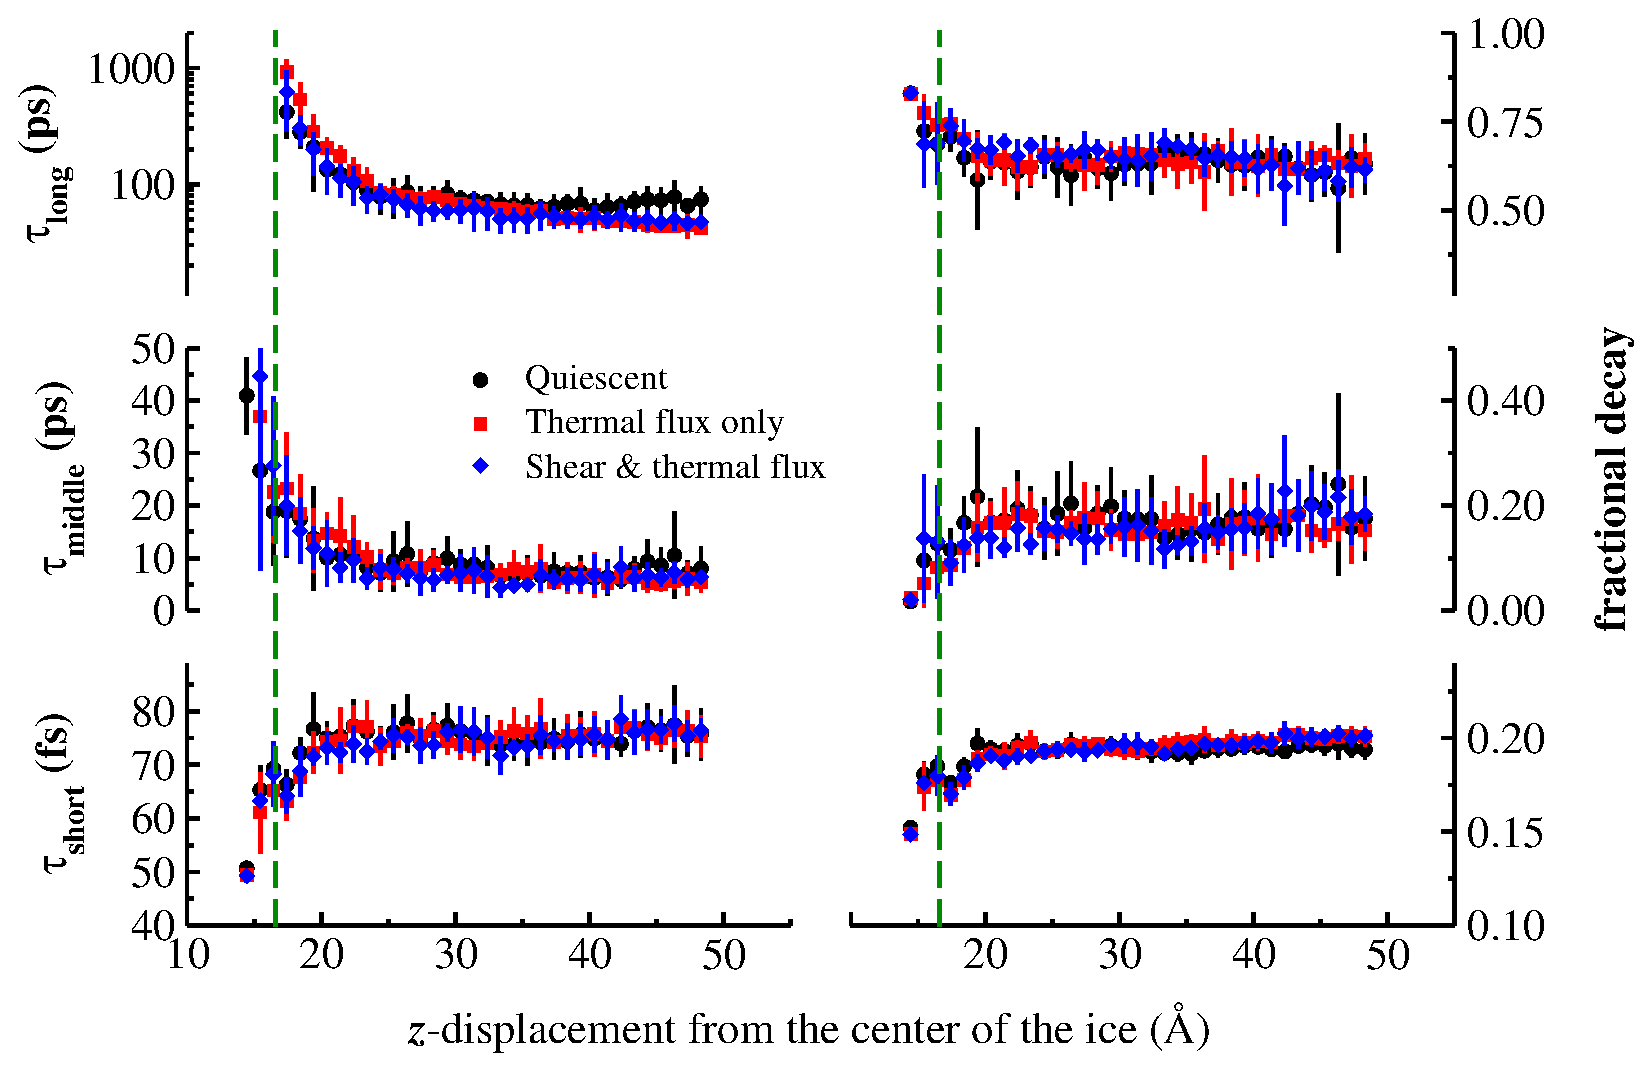
\includegraphics[width=\linewidth]{Figures/Bas_lcorrz}
\caption{\label{fig:Borient} $C_2(z,t)$ time constants for the basal
  interface.  Panel descriptions are the same as in
  Fig. \ref{fig:Pyrorient}. }
\end{figure}

\begin{figure}
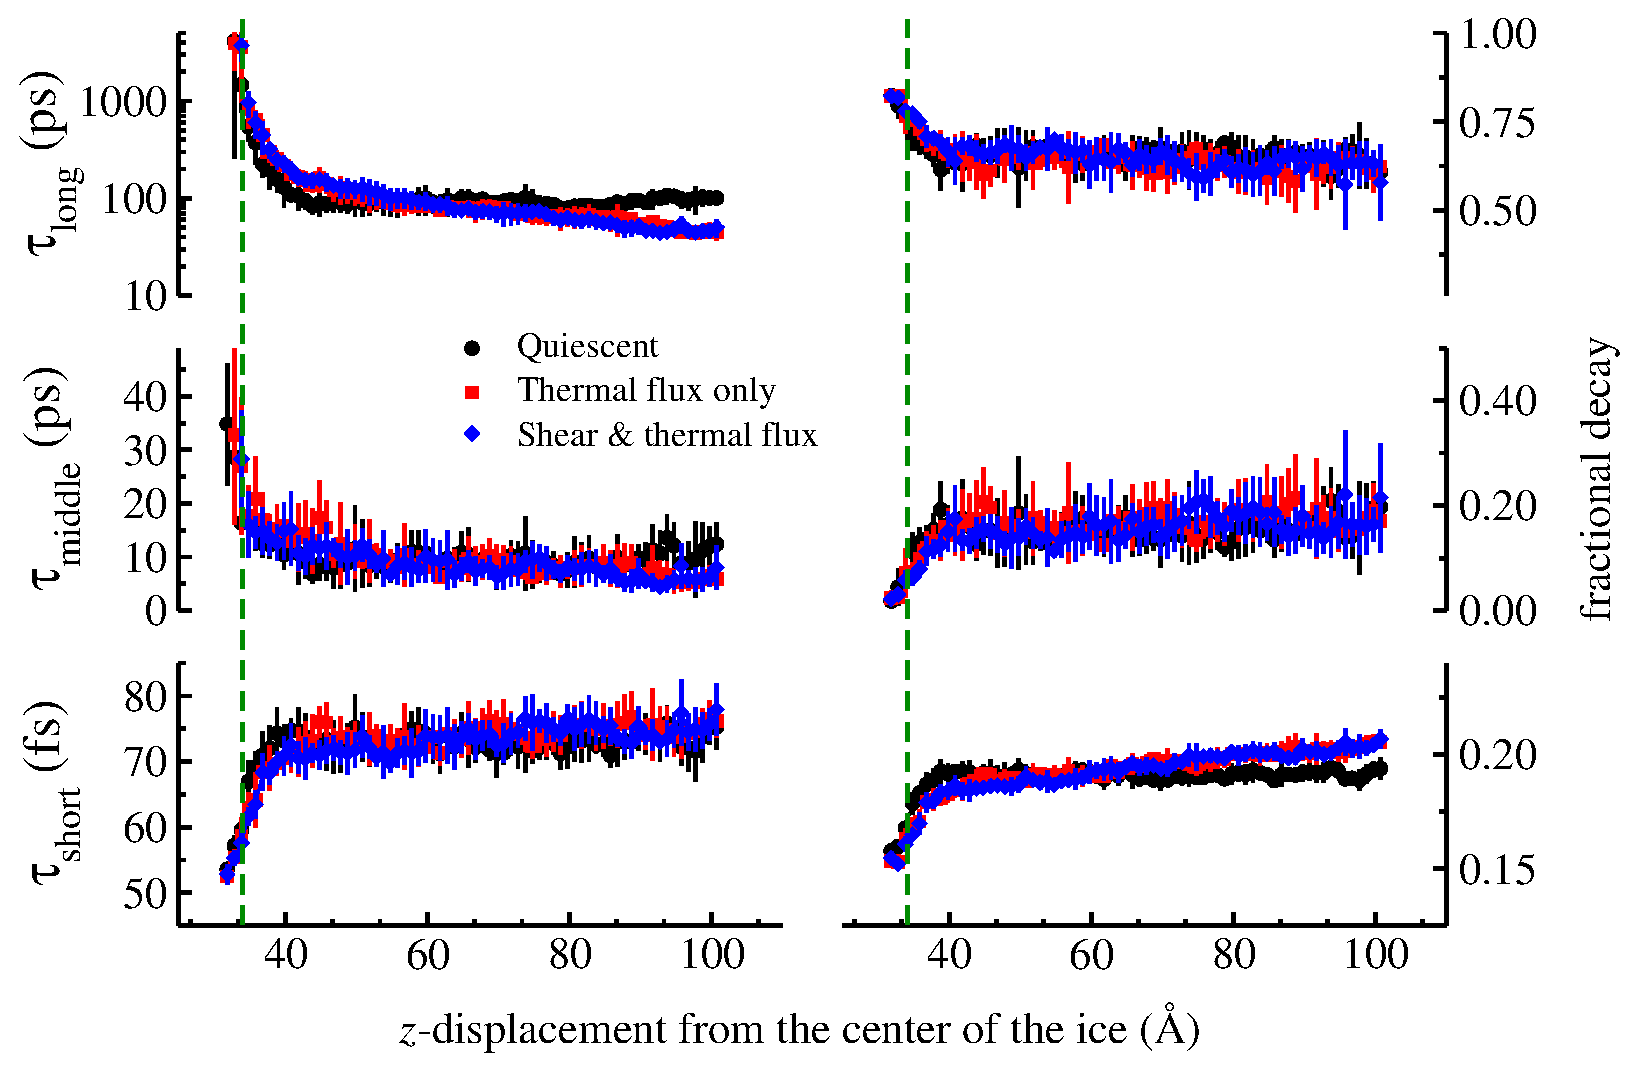
\includegraphics[width=\linewidth]{Figures/Pri_lcorrz}
\caption{\label{fig:Porient} $C_2(z,t)$ time constants for the prismatic
  interface.  Panel descriptions are the same as in
  Fig. \ref{fig:Pyrorient}.}
\end{figure}
%End z-orientation times                                                           
\begin{figure}
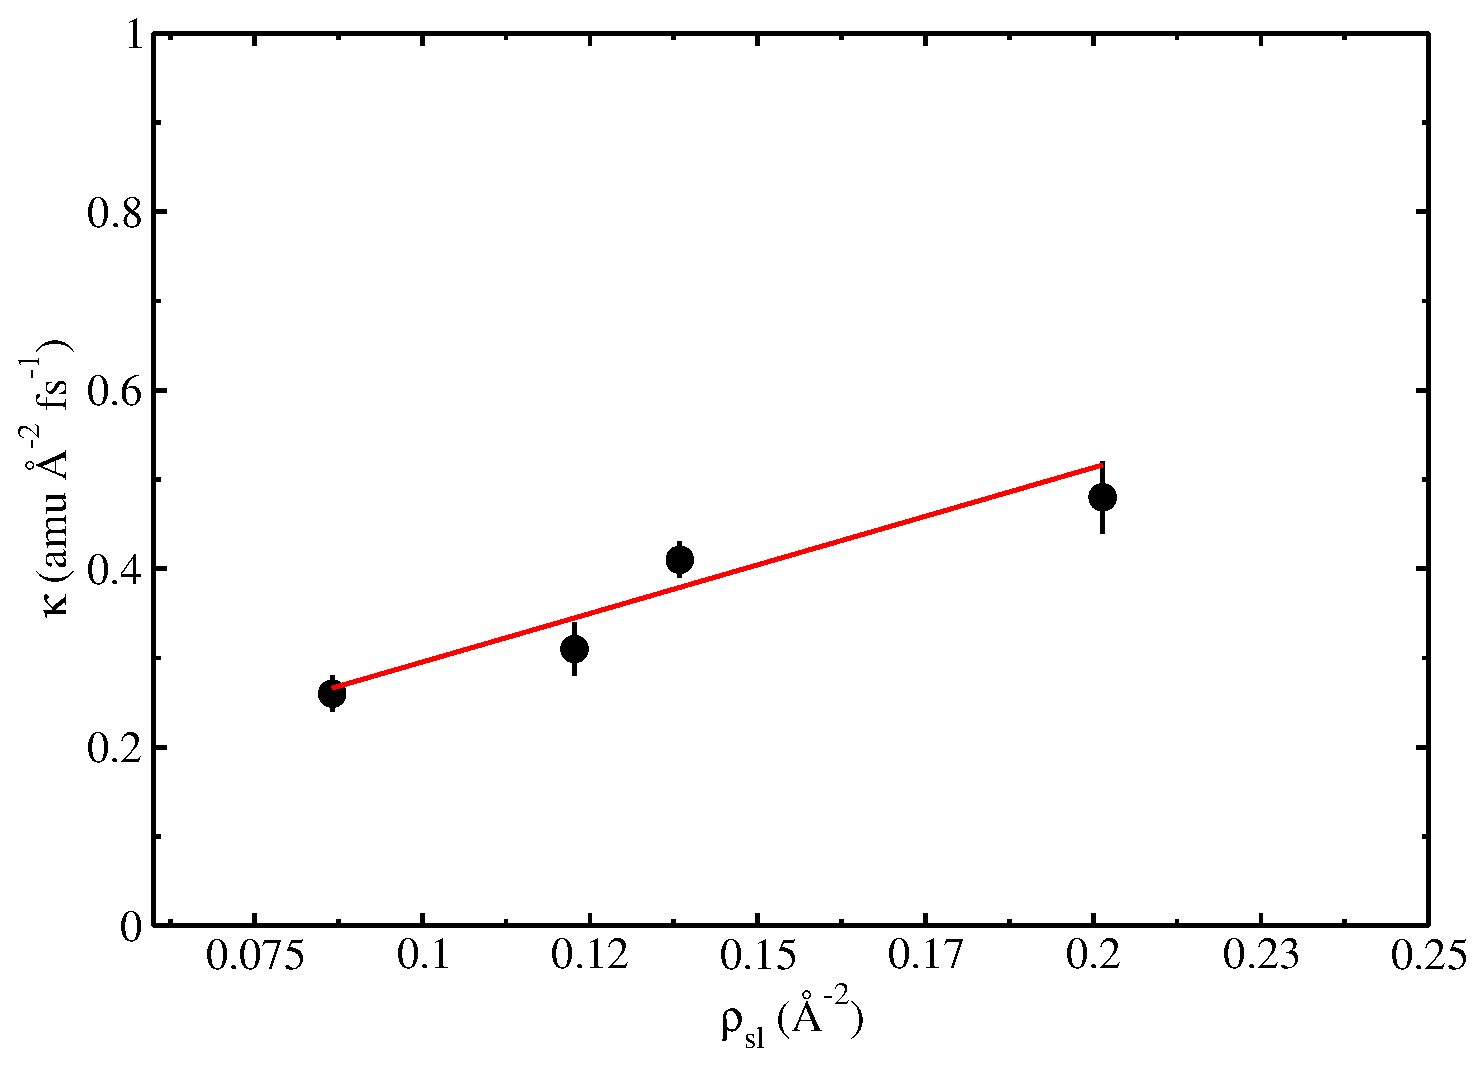
\includegraphics[width=\linewidth]{Figures/hb}
\caption{\label{fig:hbPlot} Solid-liquid friction coefficients by the
  surface density of hydrogen bonds. Linear regression gives a slope
  of 2.1772~(amu~fs\textsuperscript{-1}) and a y-intercept of
  0.0777~(amu~\AA\textsuperscript{-2}~fs\textsuperscript{-1}).} 
\end{figure}                                            
